\documentclass[a4paper, oneside, english]{sapthesis}
% add noexaminfo to the options to hide information about graduation seession

% Sapthesis explicitely loads the packages:
% xkeyval, etoolbox, geometry, ifxetex, xltxtra, fontenc, textcomp,
% lmodern, caption, graphicx, color, booktabs, amsmath, fancyhdr.
% DO NOT include them again.

\usepackage[hidelinks]{hyperref}
\usepackage{amssymb}
\usepackage{comment}
\usepackage{booktabs}
\usepackage{multirow}
\usepackage{caption}
\usepackage{xcolor}
\usepackage{subcaption}
%\usepackage{arydshln} % to use dashed lines in tables

\definecolor{customgreen}{HTML}{00B050} % 92DD5F

\renewcommand{\bibname}{References} % change Bibliography title to References

\title{Benchmarking CLIP Models for Remote Sensing \\Applications}
%\subtitle{...}
\author{Cristiana Di Tullio}
\IDnumber{1803880}
\course{Master's Degree in Data Science}
\courseorganizer{Facoltà di Ingegneria dell'Informazione, Informatica e Statistica}
\AcademicYear{2024/2025}
\advisor{Simone Scardapane}
\coadvisor{Marco Montagna}
\examdate{18th July 2025}
\examiner[]{Pierpaolo Brutti} % use [] to specify role (default:chairman)
\examiner{Mattia Crespi}
\examiner{D'Ecclesia Rita Laura}
\examiner{Francesco Leotta}
\examiner{Pompeo Polito}
\examiner{Walter Quattrociocchi}
\examiner{Simone Scardapane}
\thesistype{Master thesis}
\copyyear{2025}
\authoremail{ditullio.1803880@studenti.uniroma1.it}
\date{\today}

\begin{document}

\frontmatter
\maketitle
\dedication{(add a dedication)}

%\abstract{(add an abstract)}
\begin{abstract}
    (add an abstract)
\end{abstract}

\tableofcontents

\mainmatter

\chapter{Introduction} % -------------------------------------
% l'argomento è machine learning (SSL)
% research questions e contributi finali (sorta di anticipo delle conclusioni)
% riassunto del lavoro svolto (abstract-style)


\chapter{Related Works} % --------------------------------------
\section{CLIP in Remote Sensing}
\section{RGB approaches}

Mention all the clip models finetuned on Remote sensing images introduced so far, the ones based on the original clip (and therefore RGB-only): RemoteCLIP, GeoRSCLIP, SkyCLIP, RS-M-CLIP, all based on the same kind of "approach" (finetuning CLIP on the dataset of interest, much more work on dataset collection (which is fundamental, but works less on the model itself, more data analysis and preprocessing), then of course they try out different finetuning techniques more or less efficient parameter-wise, but if we want to keep an eye on the model size and training feasibility this is not doable - good to work on options that can be adopted on middle-standard hardware, or in situations where not much processing capability/memory is available).

-> Mention the models and the approach in general, but explain the ones used in the CLIP for RS section!!



\section{MSI approaches}

[Mainly represented by the IBM paper, explain the methodology adopted and their results, again very good job but computationally demanding. We are investigating more lightweight solutions from an engineering perspective.]


\section{Fine-Tuning techniques}

[List and describe a bit the techniques adopted in the previously discussed papers and approaches, also have a look at the ones present in the paper by that swiss guy who recently graduated with a thesis carried out in the IBM team!!]


\chapter{Vision Language Models}  % ---------------------------
Vision Language Models explained on HF: https://huggingface.co/blog/vlms

%\section{Residual Networks backbone (ResNet)}
%\subsection{Convolutional Neural Networks}
%\subsection{The ResNet architecture}

%\section{Vision Transformer backbone (ViT)}
%\subsection{The Transformers architecture}
%\subsection{The Multi-Head Self-Attention mechanism}

\chapter{The CLIP model} % ------------------------------------


The OpenAI's CLIP (Contrastive Language-Image Pre-Training) model \cite{radford2021learning} represents a significant leap in Vision-Language modeling, designed to learn a unified representation of images and texts. By jointly training on a diverse dataset of images and their corresponding textual descriptions, CLIP encodes both modalities into a shared embedding space. This shared space allows CLIP to perform zero-shot classification, text-to-image retrieval, and other cross-modal tasks without requiring task-specific fine-tuning.

The core principle behind CLIP is \emph{contrastive learning}, where the model is trained to maximize the similarity between matching image-text pairs and minimize the similarity for mismatched pairs. This approach enables the model to generalize to unseen data and tasks, making it highly versatile for real-world applications. Figure \ref{fig:clip-architecture} shows the overall structure of OpenAI's CLIP model:



\section{The CLIP architecture}

%template to add images
\begin{figure}[h]
    \centering
    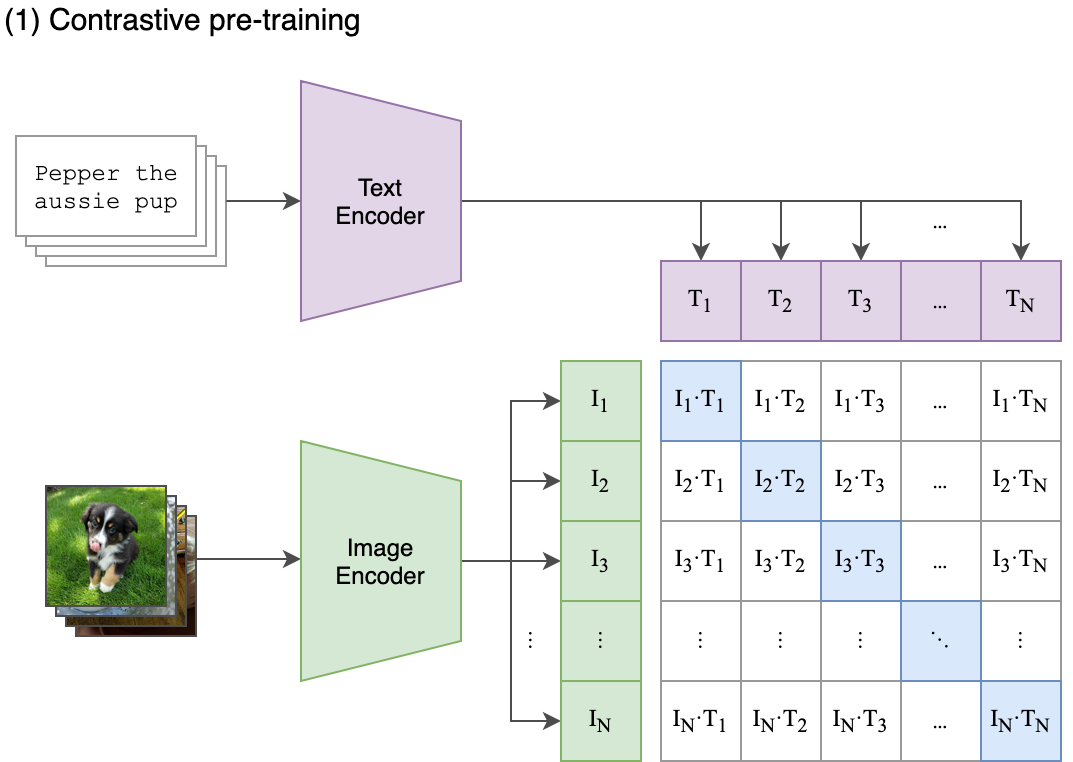
\includegraphics[width=\textwidth]{img/CLIP-structure.png}
    \caption{The CLIP model is composed by two encoders for the two different data sources, visual and textual, and employs a contrastive loss function to project the embedding of different modalities into a shared embedding space.}
    \label{fig:clip}
\end{figure}

\begin{figure}[h]
    \centering
    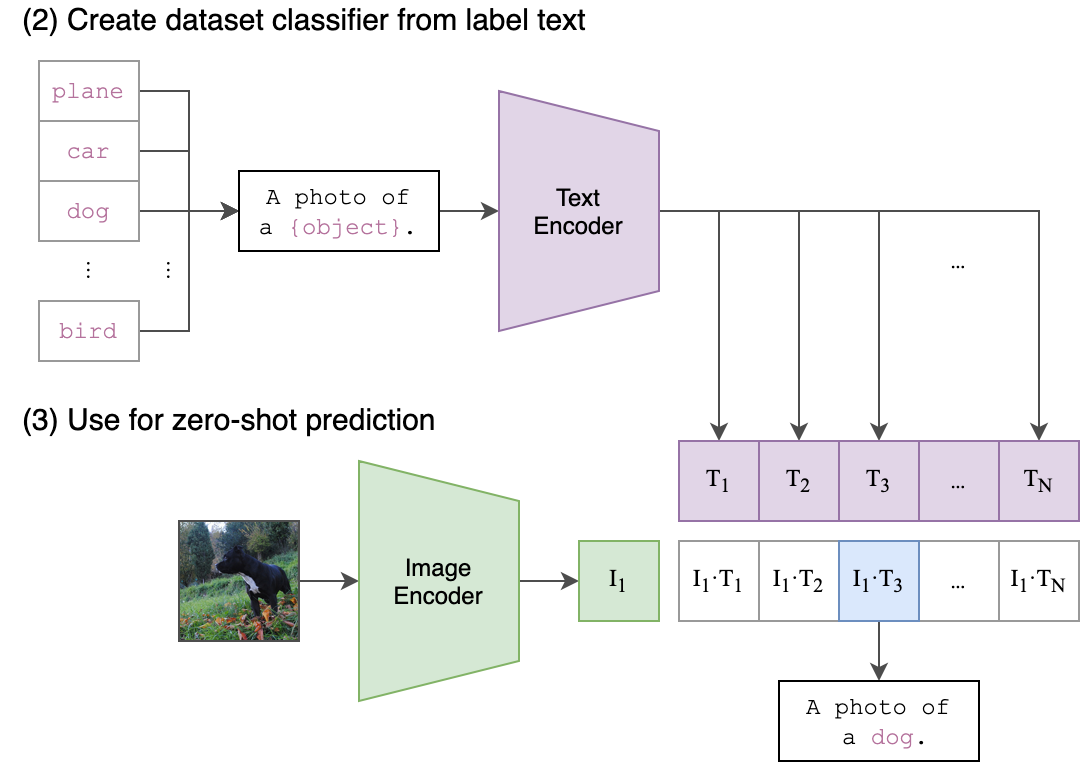
\includegraphics[width=\textwidth]{img/CLIP-zero-shot.png}
    \caption{When using CLIP for zero-shot inference, a user can feed the model custom text and image inputs and obtain similarity scores that quantify how relevant each instance of one modality is to the other.}
    \label{fig:clip-zs}
\end{figure}


\section{Contrastive Learning}
\section{Zero-Shot capabilities}

\section{CLIP-like models for Remote Sensing}

\subsection{RemoteCLIP}

\subsection{GeoRSCLIP}

\subsection{SkyCLIP}


CLIP \cite{radford2021learning} \\

(from CLIP's paper) \\

Looking at where zero-shot CLIP notably underperforms we see that zero-shot CLIP is quite weak on several specialized, complex, or abstract tasks such as satellite image classification (EuroSAT and RESISC45), lymph node tumor detection (PatchCamelyon), counting objects in synthetic
scenes (CLEVRCounts), self-driving related tasks such as German traffic sign recognition (GTSRB), recognizing distance to the nearest car (KITTI Distance). These results highlight the poor capability of zero-shot CLIP on more complex tasks. \\

Finally, we found that on satellite image classification datasets it helped to specify that the images were of
this form and we use variants of "a satellite photo
of a {label}."


\chapter{Datasets} % ------------------------------------------

A note before proceeding: the following datasets have been adopted due to their nature of benchmark and their importance in the literature, but they are *not* proper image-text datasets (that would be the best option to work with CLIP). This limitation is partly reflected in the final results, but they don't invalidate this work's contribution 

\section{EuroSAT}

EuroSAT \cite{helber2019eurosat} is possibly the most well known dataset in Earth Observation ground/benchmark/ studies, has been the beta-tester for all the experiments carried out in this project and the main evaluation reference to compare models performance, even if it's less diverse and comprehensive than GEO-Bench (not as complete as a benchmark) it's been around for more time and many more experiments have been carried out on it, so good for reference as well.

\begin{figure}[h]
    \centering
    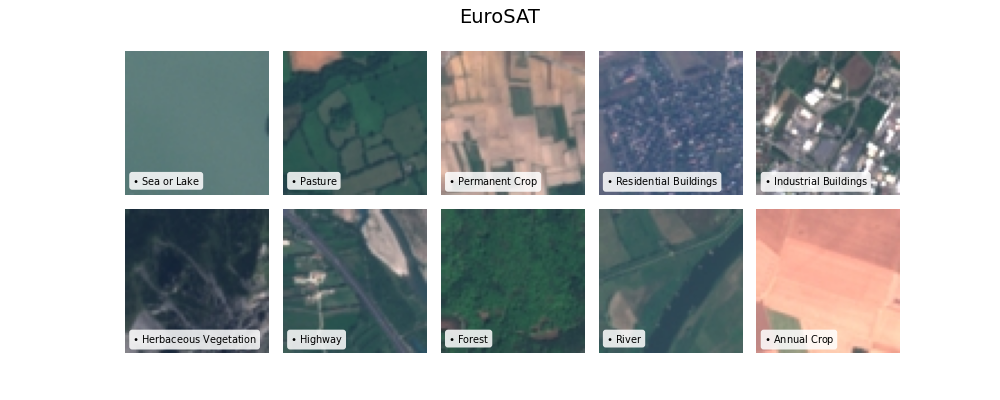
\includegraphics[width=\textwidth]{img/EuroSAT_image_grid.png}
    \caption{Sample images from the 10 classes contained in the EuroSAT original dataset.}
    \label{fig:eurosatgrid}
\end{figure}


\paragraph{Characteristics}


\begin{table}[ht]
\centering
\footnotesize
\renewcommand{\arraystretch}{1.2}
    \begin{tabular}{rcccccclcl}
    \toprule
    Name & Image Size & \# Classes & Train & Val & Test & \# Bands & RGB res & Sensors  \\
    \midrule
    EuroSAT & & 10 & 10000 & 5000 & 5000 & 13 & & Sentinel-2 \\
    \bottomrule
    \end{tabular}
\vspace{0.3cm}
\caption{\normalsize EuroSAT dataset characteristics.}
\label{tab:classtypes}
\end{table}


\paragraph{Composition}

\section{GEO-Bench}

The GEO-Bench dataset collection \cite{lacoste2023geo} was presented in 2023 with the purpose of .... . Its global samples span across different countries and continents, as shown in Figure \ref{fig:geoworld}. The main characteristics of the datasets of interest are summarized in the table below. 

\begin{figure}[h]
    \centering
    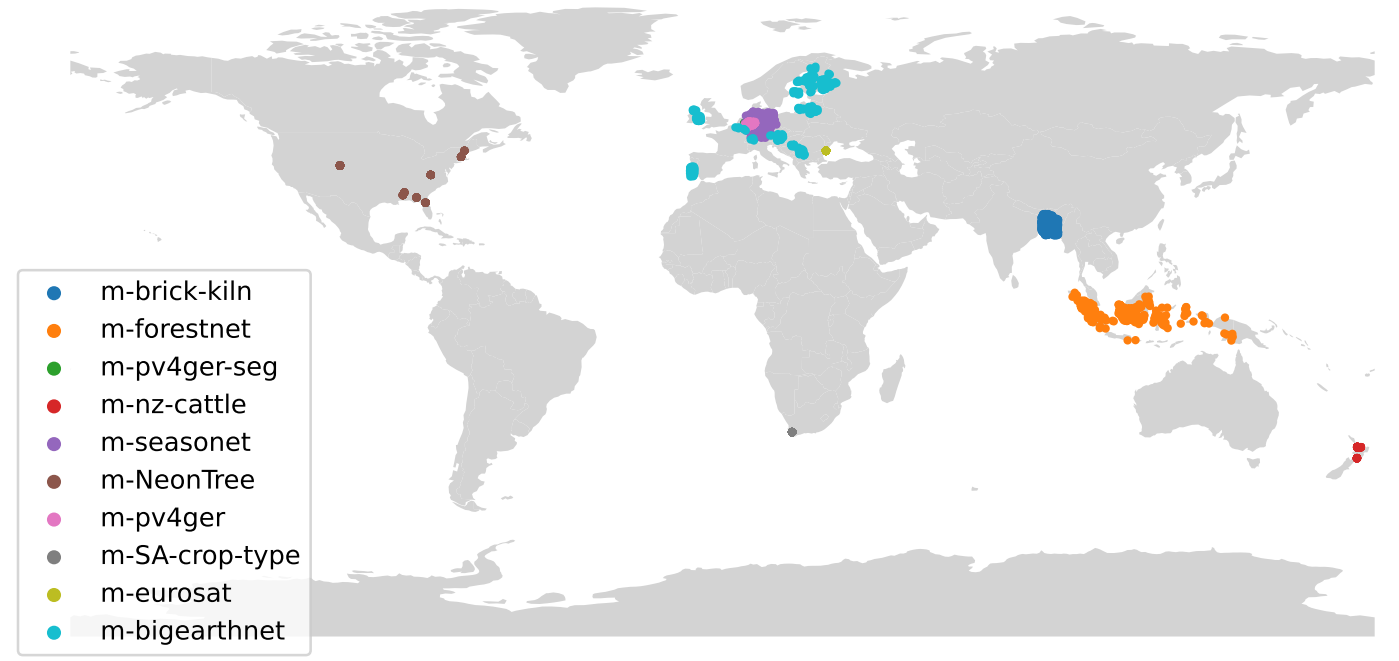
\includegraphics[width=0.6\textwidth]{img/geobench_world_coverage.png}
    \caption{The world coverage of different datasets of the benchmark, as reported in \cite{lacoste2023geo}.}
    \label{fig:geoworld}
\end{figure}

\paragraph{Composition}

The benchmark comprises six image classification datasets and six image segmentation datasets. For the purposes of this project, we will only focus on the \emph{classification} ones, a brief illustration of which follows below: \\

\begin{figure}[h]
    \centering
    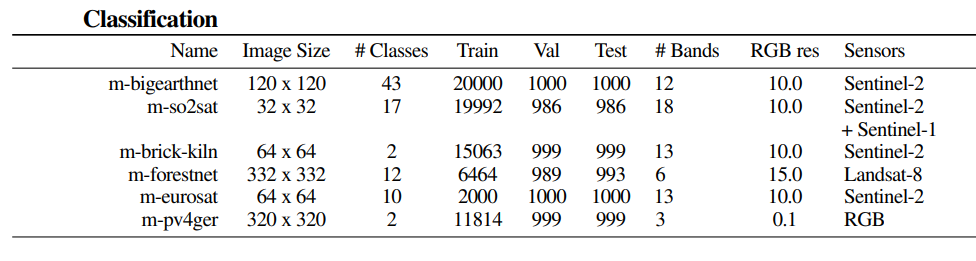
\includegraphics[width=\textwidth]{img/geobench-datasets-classification-info-cut.png}
    \caption{Characteristics of datasets in the benchmark \cite{lacoste2023geo}.}
    \label{fig:geoinfo}
\end{figure}

[List classification datasets one by one with small description, see the links in the notebook for more information and context] 


\paragraph{Diversity of Imagery} The datasets contain images acquired with different satellite sensors and preprocessed by different technologies, resulting in images with different size, resolution, and available spectral bands.


\paragraph{Diversity of Classification Tasks} The classification datasets are the result of different studies conducted with different purposes, therefore they are associated to a different kind of classification tasks. Except for the binary case, the other tasks vary greatly in number and type of classes, and these differences are outlined in Table \ref{tab:classtypes}. Here, "short captions" identifies class names identified by $2-3$ words at most, while "caption" refers to class names identified by $>5$ words, and "words" trivially refers to class names identified by single words.


\begin{table}[ht]
\centering
\footnotesize
\renewcommand{\arraystretch}{1.2}
    \begin{tabular}{lcccc}
    \toprule
    \textbf{Dataset} & \textbf{Origin} & \textbf{Classification task} & \textbf{\# Classes} & \textbf{Type of classes}  \\
    \midrule
    m-brick-kiln & GEO-Bench & binary & 2 & short captions \\
    m-pv4ger & GEO-Bench & binary & 2 & short captions \\
    m-forestnet & GEO-Bench & multiclass & 12 & words \\
    m-eurosat & GEO-Bench & multiclass & 10 & words \\
    m-so2sat & GEO-Bench & multiclass & 17 & words \\
    m-bigearthnet & GEO-Bench & multilabel & 43 & captions \\
    \bottomrule
    \end{tabular}
\vspace{0.3cm}
\caption{\normalsize Classification task details for every dataset analyzed.}
\label{tab:classtypes}
\end{table}


\subsection{m-brick-kiln}


\begin{figure}[h]
    \centering
    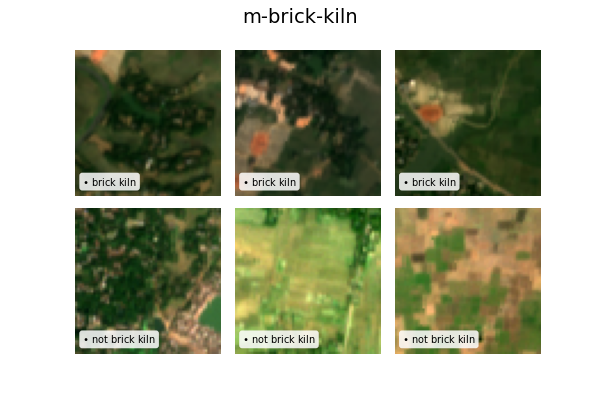
\includegraphics[width=0.7\textwidth]{img/m-brick-kiln_image_grid.png}
    \caption{Sample images from the 2 classes contained in the m-brick-kiln dataset from GEO-Bench.}
    \label{fig:brickgrid}
\end{figure}


\subsection{m-pv4ger}

\begin{figure}[h]
    \centering
    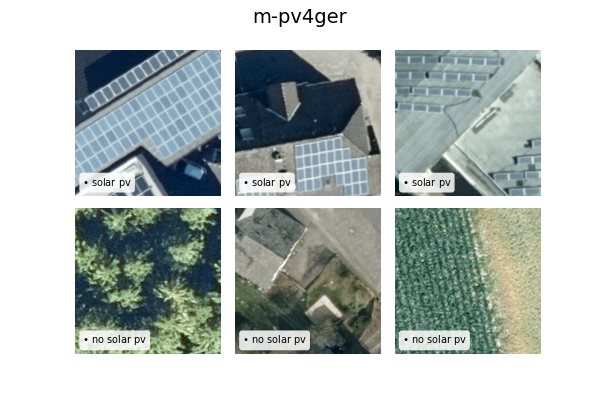
\includegraphics[width=0.7\textwidth]{img/m-pv4ger_image_grid.png}
    \caption{Sample images from the 2 classes contained in the m-pv4ger dataset from GEO-Bench.}
    \label{fig:solargrid}
\end{figure}


\subsection{m-forestnet}


\begin{figure}[h]
    \centering
    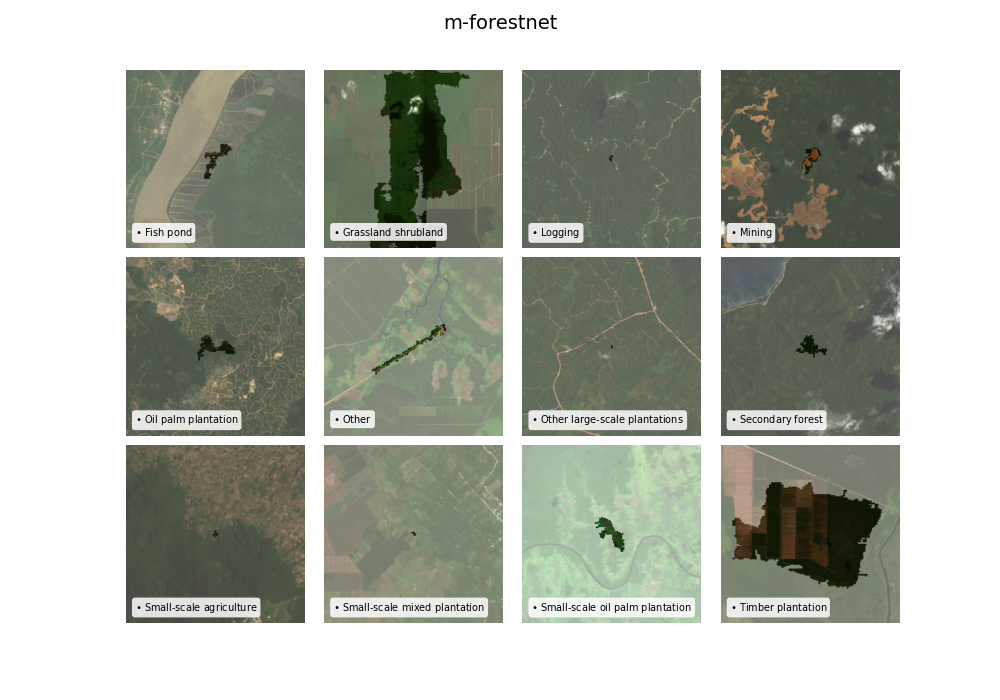
\includegraphics[width=0.8\textwidth]{img/m-forestnet_image_grid.png}
    \caption{Sample images from the 12 classes contained in the m-forestnet dataset from GEO-Bench.}
    \label{fig:forestnetgrid}
\end{figure}


\subsection{m-eurosat}

Specify how this dataset was preprocessed and modified, highlight differences wrt the original EuroSAT


\begin{figure}[h]
    \centering
    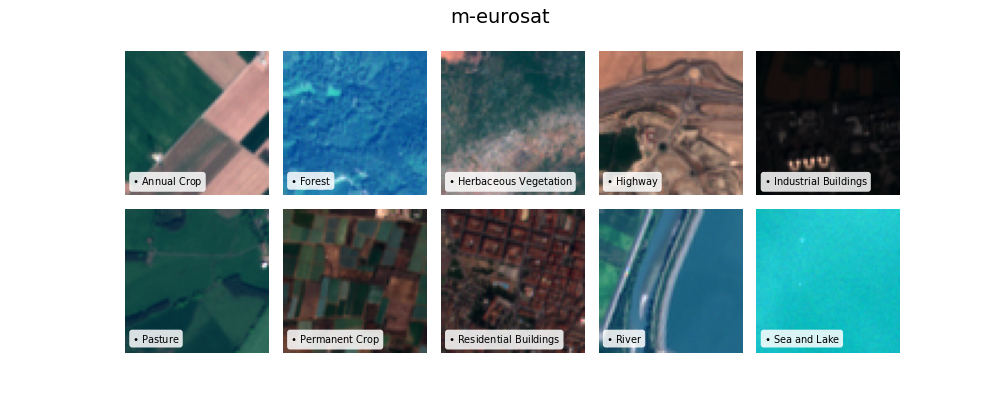
\includegraphics[width=\textwidth]{img/m-eurosat_image_grid.png}
    \caption{Sample images from the 10 classes contained in the m-eurosat dataset from GEO-Bench.}
    \label{fig:meurosatgrid}
\end{figure}


\subsection{m-so2sat}


\begin{figure}[h]
    \centering
    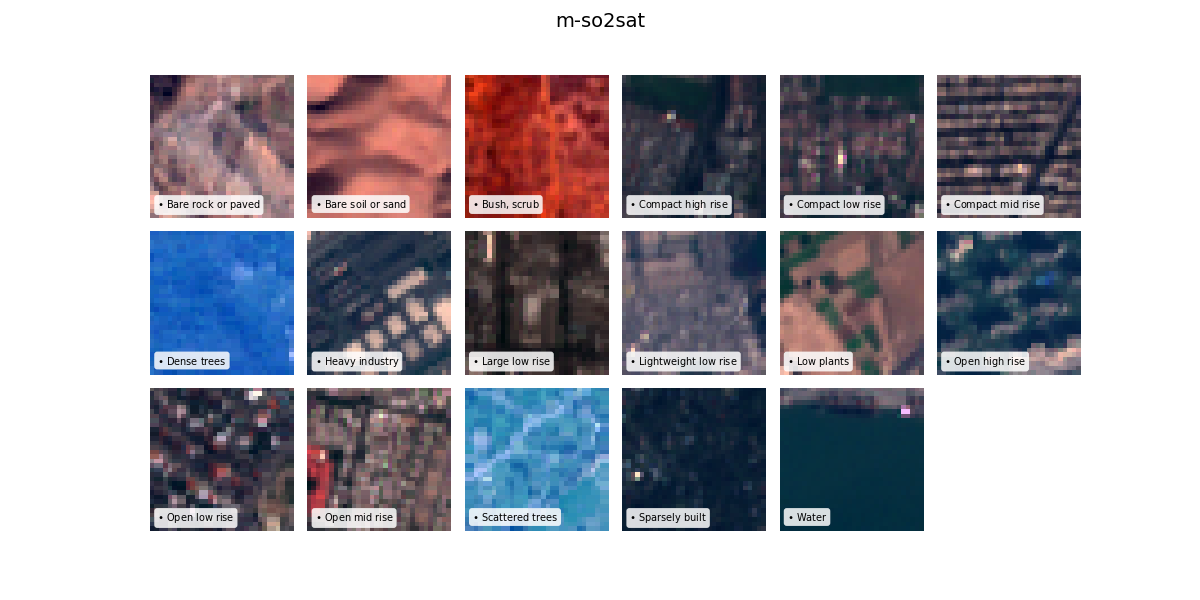
\includegraphics[width=\textwidth]{img/m-so2sat_image_grid.png}
    \caption{Sample images from the 17 classes contained in the m-so2sat dataset from GEO-Bench.}
    \label{fig:so2satgrid}
\end{figure}


\subsection{m-bigearthnet}


\begin{figure}[h]
    \centering
    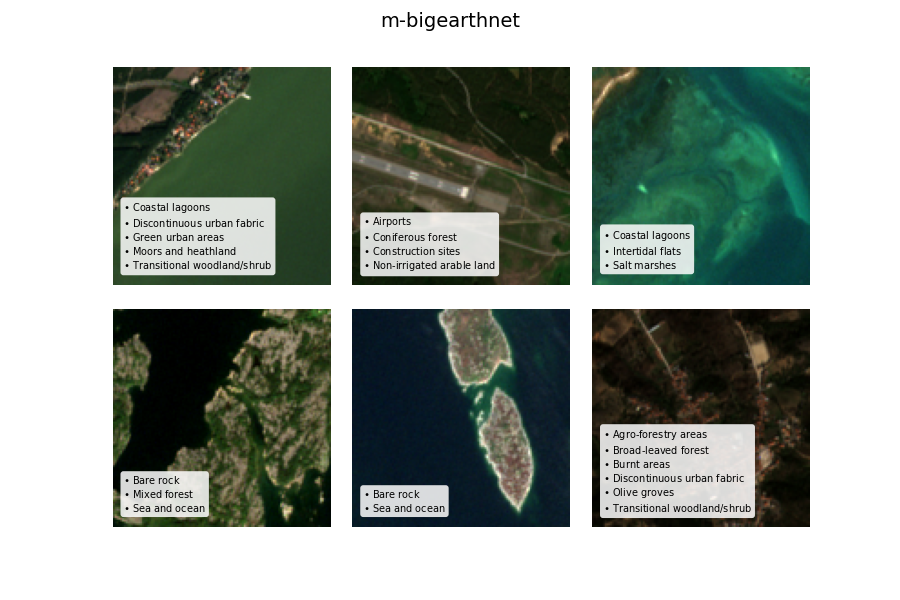
\includegraphics[width=\textwidth]{img/m-bigearthnet_image_grid.png}
    \caption{Sample multilabel images featured in the m-bigearthnet dataset from GEO-Bench.}
    \label{fig:bengrid}
\end{figure}


\chapter{Approach} % ------------------------------------------

\section{Multi Spectral Embedders}

\subsection{MSI-1 embedder}
\subsection{MSI-2 embedder}
\subsection{MSI-T embedder}

\section{MSI + CLIP Model Structure}

\paragraph{Base model}
\paragraph{Transfer Learning model}

\chapter{Experimental setup} % --------------------------------

This project focuses on some ground benchmarking work in the scope of \emph{image classification}. This task has been chosen for reasons like a lack of baseline results to compare CLIP-like models to different types of VLMs, but also between themselves. Given the versatility of these models and the possible application to several types of tasks, the literature disagrees/is not uniform in the tasks (and consequentially in the evaluation) of these models. For simplicity, and to make the results more significant in the context of existing literature, and to fill small research gaps that miss a comprehensive evaluation of these models, we choose here to focus on classification (also for the "universality" of this task, it's easy to understand, it's easy to compare models on it). Therefore, we adopt the classic classification evaluation metrics for the binary and multiclass tasks, while some more research has been carried out to evaluate the multilabel task as it needs to be treated a bit differently.

\section{Evaluation metrics}

\paragraph{Binary/Multiclass Classification}

\begin{itemize}
    \item \textbf{Accuracy}:
    \item \textbf{Precision}:
    \item \textbf{Recall}:
    \item \textbf{F1 Score}:
    \item \textbf{Confusion Matrix}
\end{itemize}

\paragraph{Multilabel Classification}

\begin{itemize}
    \item \textbf{Precision@k (P@k)}:
    \item \textbf{Recall@k (R@k)}:
    \item \textbf{Mean Average Precision (mAP)}:
    \item \textbf{Micro F1}:
    \item \textbf{Ranking Loss}:
\end{itemize}


\section{Baseline tests}

\paragraph{EuroSAT}

\begin{table}[h]
\centering
\footnotesize
\renewcommand{\arraystretch}{1.2}
    \begin{tabular}{llc}
    \specialrule{.1em}{.2em}{.2em}
    \textbf{Model} & \textbf{Backbone} & \textbf{EuroSAT} \\
    \specialrule{.06em}{.2em}{.2em}
    CLIP        & ViT-B/32 & 38.76\% \\ 
    RemoteCLIP  & ViT-B/32 & 37.34\% \\
    GeoRSCLIP   & ViT-B/32 & \textbf{53.54\%} \\
    SkyCLIP     & ViT-B/32 & 52.26\% \\
    \specialrule{.1em}{.2em}{.2em}
    \end{tabular}
\vspace{0.3cm}
\caption{\normalsize Comparison of zero-shot accuracies obtained by different models on the EuroSAT original dataset.}
\label{tab:eurobaselines}
\end{table}


\begin{figure}[h]
  \begin{subfigure}[t]{.5\textwidth}
    \centering
    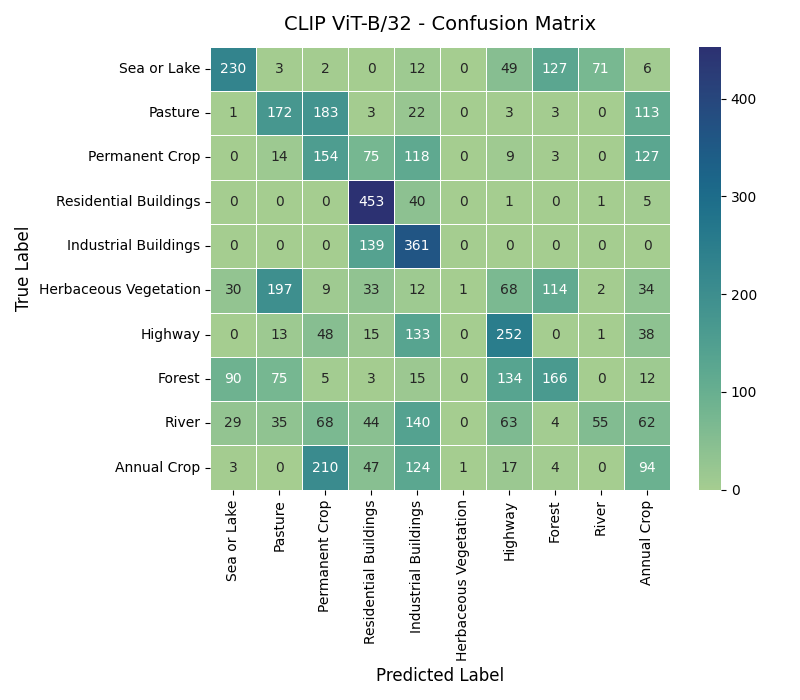
\includegraphics[width=\linewidth]{img/EuroSAT_CLIP_32_cm.png}
    %\caption{}
  \end{subfigure}
  \hfill
  \begin{subfigure}[t]{.5\textwidth}
    \centering
    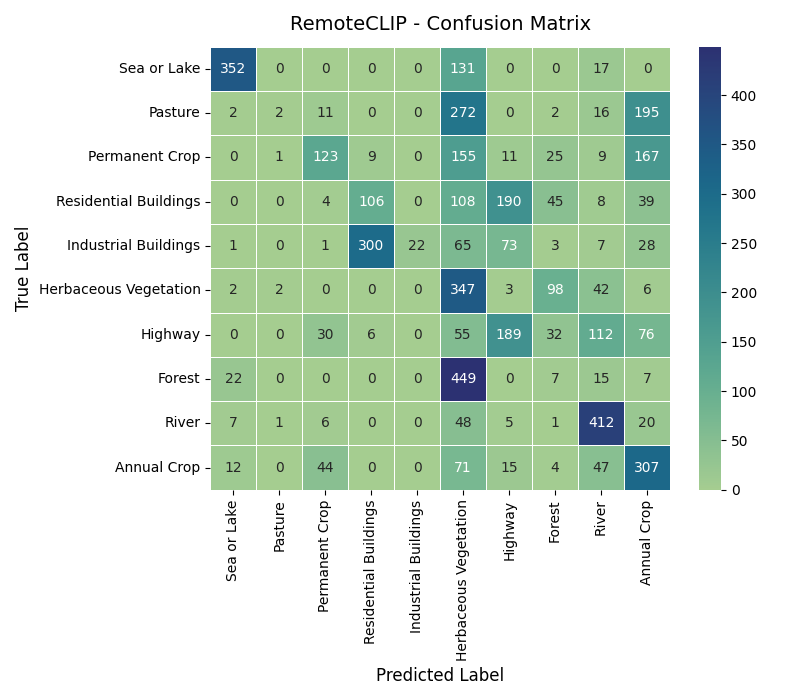
\includegraphics[width=\linewidth]{img/EuroSAT_RemoteCLIP_32_cm.png}
    %\caption{}
  \end{subfigure}

  \medskip

  \begin{subfigure}[t]{.5\textwidth}
    \centering
    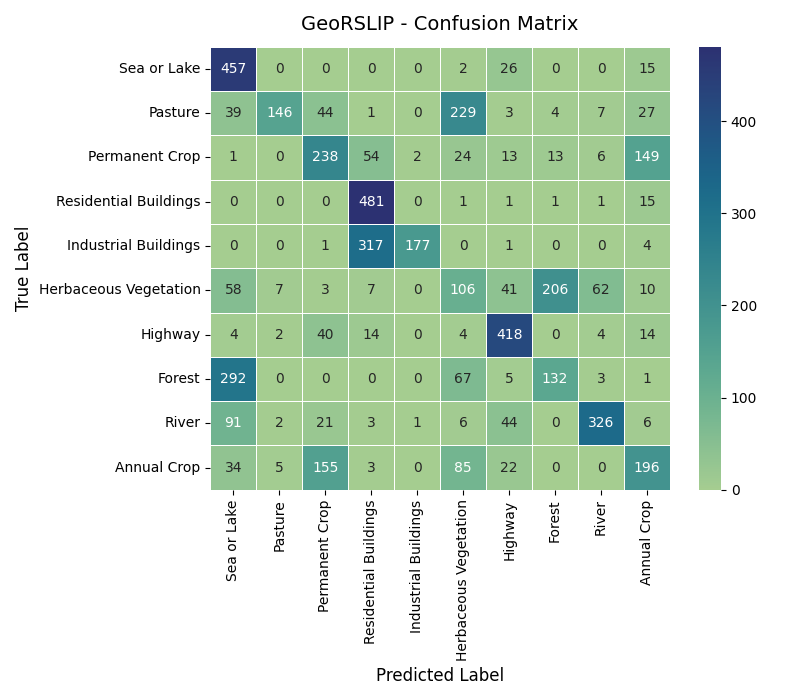
\includegraphics[width=\linewidth]{img/EuroSAT_GeoRSCLIP_32_cm.png}
    %\caption{}
  \end{subfigure}
  \hfill
  \begin{subfigure}[t]{.5\textwidth}
    \centering
    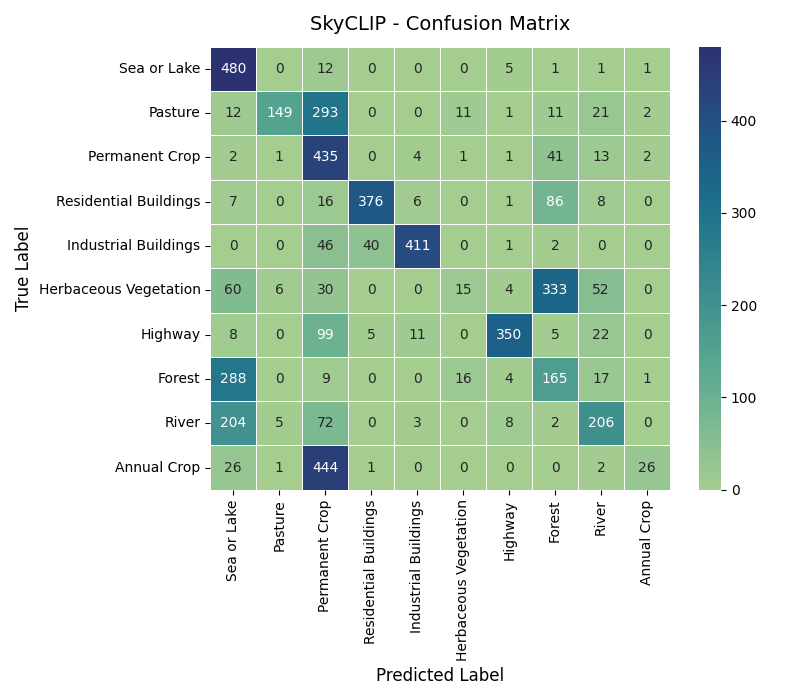
\includegraphics[width=\linewidth]{img/EuroSAT_SkyCLIP_32_cm.png}
    %\caption{}
  \end{subfigure}
  \caption{Confusion matrices of CLIP and other CLIP-like models finetuned on Remote Sensing datasets, evaluated on EuroSAT: while CLIP and RemoteCLIP's matrices appear somewhat fuzzy and struggle to recognize some classes at all, GeoRSCLIP and SkyCLIP's ones feature a more definite diagonal.}
\end{figure}



\paragraph{GEO-Bench}


\begin{table}[ht]
\centering
\footnotesize
\renewcommand{\arraystretch}{1.2}
    \begin{tabular}{llccccc}
    %\hline
    \specialrule{.1em}{.2em}{.2em}
    \textbf{Model} & \textbf{Backbone} & \textbf{m-brick-kiln} & \textbf{m-pv4ger} & \textbf{m-forestnet} & \textbf{m-eurosat} & \textbf{m-so2sat} \\
    %{} & {} & \textbf{acc} & \textbf{acc} & \textbf{acc} & \textbf{acc} & \textbf{acc} \\
    %\hline
    \specialrule{.06em}{.2em}{.2em}
    CLIP        & ViT-B/32 & \textbf{70.27\%} & 73.87\% & 7.65\% & 41.90\% & \textbf{16.63\%}\\ %\hdashline[2pt/5pt]
    RemoteCLIP  & ViT-B/32 & 66.97\% & 65.97\% & 8.25\% & 28.70\% & 12.78\% \\
    GeoRSCLIP   & ViT-B/32 & 68.67\% & 89.09\% & \textbf{14.20\%} & \textbf{51.30\%} & 15.82\% \\
    SkyCLIP     & ViT-B/32 & 59.36\% & \textbf{90.59\%} & 10.67\% & 49.30\% & 12.27\% \\
    %\hline
    \specialrule{.1em}{.2em}{.2em}
    \end{tabular}
\vspace{0.3cm}
\caption{\normalsize Comparison of zero-shot accuracies obtained by different models across GEO-Bench datasets.}
\label{tab:baselines}
\end{table}


\begin{table}[ht]
\centering
\footnotesize
\renewcommand{\arraystretch}{1.2}
    \begin{tabular}{llcccc|c}
    \toprule
    %\textbf{Model} & \textbf{Method} & \multicolumn{5}{c}{\textbf{m-bigearthnet}} \\
    \multirow{2}{*}{\textbf{Model}} & \multirow{2}{*}{\textbf{Backbone}} & \multicolumn{5}{c}{\textbf{m-bigearthnet}} \\
    \cmidrule(lr){3-7}
    & & \textbf{R@5} & \textbf{P@5} & \textbf{mAP} & \textbf{F1} & \textbf{rloss} \\
    \specialrule{.06em}{.2em}{.2em}
    CLIP        & ViT-B/32 & 31.70\% & 23.40\% & 32.32\% & 20.39\% & 28.71\% \\ 
    RemoteCLIP  & ViT-B/32 & 26.24\% & 19.82\% & 27.63\%  & 20.30\% & 30.89\%  \\
    GeoRSCLIP   & ViT-B/32 & \textbf{38.89\%} & \textbf{28.60\%} & \textbf{39.69\%} & 22.15\% & \textbf{23.19\%} \\
    SkyCLIP     & ViT-B/32 & 26.53\% & 19.30\% & 28.61\% & \textbf{22.39\%} & 30.98\%  \\
    \bottomrule
    \end{tabular}
\vspace{0.3cm}
\caption{\normalsize Comparison of zero-shot performance metrics obtained by different models on the m-bigearthnet dataset from GEO-Bench.}
\label{tab:baselines-multilab}
\end{table}


\section{Text prompts experiments}

* Focus on binary classification *

- Explain the problems with negation, cite paper \cite{quantmeyer2024and}

- Explain the idea behind the binary approach and the one behind the multi-prompt approach

\paragraph{m-brick-kiln}

TODO: List the prompts and the corresponding mapping to positive/negative classes


\begin{table}[ht]
\centering
\footnotesize
\renewcommand{\arraystretch}{1.2}
    \begin{tabular}{lc|cccc}
    \toprule
    %\textbf{Model} & \textbf{original} & \textbf{Prompt 1} & \textbf{Prompt 2} & \textbf{Prompt 3} & \textbf{Multi-Prompt} \\
    \multirow{2}{*}{\textbf{Model}} & \multicolumn{4}{c}{\textbf{Binary Prompts}} &  \multirow{2}{*}{\textbf{Multi-Prompt}}\\
    \cmidrule(lr){2-5}
    & \textbf{Original} & \textbf{Type 1} & \textbf{Type 2} & \textbf{Type 3} \\
    \midrule
    CLIP & 70.27\% & 76.58\% & 80.38\% & 79.78\% & \textbf{83.58\%} \\
    RemoteCLIP & 66.97\% & 66.27\% & 66.77\% & \textbf{67.47\%} & 66.57\% \\
    GeoRSCLIP & 68.67\% & 71.87\% & 70.57\% & \textbf{73.37\%} & 68.17\%\\
    SkyCLIP & 59.36\% & 69.07\% & \textbf{69.27\%} & 69.17\% & 67.57\% \\ 
    \bottomrule
    \end{tabular}
\vspace{0.3cm}
\caption{\normalsize CLIP performance on m-brick-kiln with different text prompts.}
\label{tab:prompts1}
\end{table}


\paragraph{m-pv4ger}

TODO: List the prompts and the corresponding mapping to positive/negative classes


\begin{table}[ht]
\centering
\footnotesize
\renewcommand{\arraystretch}{1.2} % increase row spacing
    \begin{tabular}{lc|cccc}
    \toprule
    %\textbf{Model} & \textbf{original} & \textbf{Prompt 1} & \textbf{Prompt 2} & \textbf{Prompt 3} & \textbf{Multi-Prompt} \\
    \multirow{2}{*}{\textbf{Model}} & \multicolumn{4}{c}{\textbf{Binary Prompts}} &  \multirow{2}{*}{\textbf{Multi-Prompt}}\\
    \cmidrule(lr){2-5}
    & \textbf{Original} & \textbf{Type 1} & \textbf{Type 2} & \textbf{Type 3} \\
    \midrule
    CLIP & 73.87\% & 71.57\% & 79.28\% & 76.78\% & \textbf{82.88\%} \\
    RemoteCLIP & 65.97\% & 45.85\% & 48.15\% & 32.03\% & \textbf{74.47\%} \\
    GeoRSCLIP & 89.09\% & \textbf{94.19\%} & 93.29\% & 93.89\% & 92.09\% \\
    SkyCLIP & 90.59\% & 91.99\% & 90.79\% & 91.59\% & \textbf{92.09\%} \\
    \bottomrule
    \end{tabular}
\vspace{0.3cm}
\caption{\normalsize CLIP performance on m-pv4ger with different text prompts.}
\label{tab:prompts2}
\end{table}


\section{Image normalization experiments}

\begin{figure}[h]
    \centering
    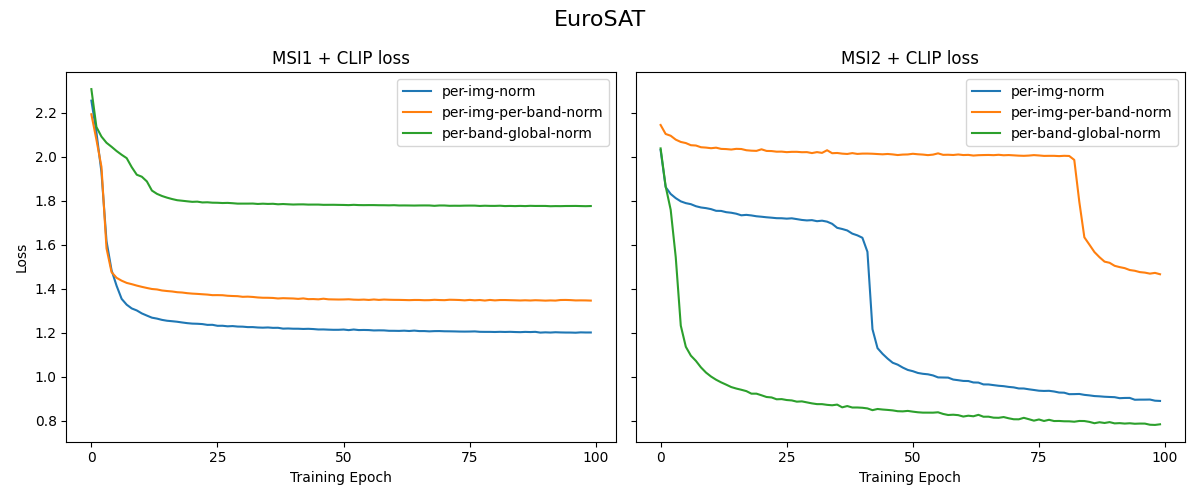
\includegraphics[width=\textwidth]{img/EuroSAT_norm_losses_plot.png}
    \caption{The effect of different normalization functions on the convergence of the training loss for the two different models.}
    \label{fig:normlosses}
\end{figure}

- comments of what normalization works best for the different models, how we calculated them, lin min max, cite \cite{unknown}, etc - 

Mention that to keep integrity and consistency with the dataset we adopt norm3 for all the following experiments and training.


\chapter{Results} % -------------------------------------------

\section{Finetuning results}


\begin{comment}
\begin{table}[ht]
\centering
\small
\renewcommand{\arraystretch}{1.2} 
    \begin{tabular}{ccccccc}
    %\hline
    \specialrule{.1em}{.2em}{.2em}
    \textbf{Model} & \textbf{Method} & \textbf{m-brick-kiln} & \textbf{m-pv4ger} & \textbf{m-forestnet} & \textbf{m-eurosat} & \textbf{m-so2sat} \\
    %\hline
    \specialrule{.06em}{.2em}{.2em}
    CLIP      & zero-shot & 70.27\% & 73.87\% & 7.65\% & 41.90\% & 16.63\% \\
    | &  | & | & | & | &| & | \\
    MSI1+CLIP & MSI1 training & 84.48\% & 87.18\% & \textbf{10.77\%} & 44.29\% & \textbf{18.96\%} \\
    {} & $\pm\Delta$ & \textcolor{customgreen}{+14.21\%} & \textcolor{customgreen}{+13.31\%} & \textcolor{customgreen}{+3.12\%} & \textcolor{customgreen}{+2.39\%} & \textcolor{customgreen}{+2.33\%} \\
    MSI2+CLIP & MSI2 training & \textbf{89.88\%} & \textbf{93.69\%} & 9.36\% & \textbf{66.79\%} & 18.35\% \\
    {} & $\pm\Delta$ & \textcolor{customgreen}{+19.62\%} & \textcolor{customgreen}{+19.82\%} & \textcolor{customgreen}{+1.71\%} & \textcolor{customgreen}{+24.89\%} & \textcolor{customgreen}{+1.72\%} \\
    %\hline
    \specialrule{.1em}{.2em}{.2em}
    \end{tabular}
\vspace{0.3cm}
\caption{Comparison of models with respect to the original CLIP.}
\label{tab:multimodal_models}
\end{table}
\end{comment}


%UPDATED:

\begin{table}[ht]
\centering
\footnotesize
\renewcommand{\arraystretch}{1.3} 
    \begin{tabular}{ccccccc}
    %\hline
    \specialrule{.1em}{.2em}{.2em}
    \textbf{Model} & \textbf{Method} & \textbf{m-brick-kiln} & \textbf{m-pv4ger} & \textbf{m-forestnet} & \textbf{m-eurosat} & \textbf{m-so2sat} \\
    %\hline
    \specialrule{.06em}{.2em}{.2em}
    CLIP      & zero-shot & 70.27\% & 73.87\% & 7.65\% & 41.90\% & 16.63\% \\
    | &  | & | & | & | &| & | \\
    MSI1+CLIP & MSI1 training & 86.38\% & 92.19\% & \textbf{10.67\%} & 44.40\% & 15.82\% \\
    {} & $\pm\Delta$ & \textcolor{customgreen}{+16.11\%} & \textcolor{customgreen}{+18.32\%} & \textcolor{customgreen}{+3.02\%} & \textcolor{customgreen}{+2.50\%} & \textcolor{red}{-0.81\%} \\
    MSI2+CLIP & MSI2 training & \textbf{90.19\%} & \textbf{92.89\%} & 9.86\% & \textbf{67.50\%} & 18.45\% \\
    {} & $\pm\Delta$ & \textcolor{customgreen}{+19.92\%} & \textcolor{customgreen}{+19.02} & \textcolor{customgreen}{+2.21\%} & \textcolor{customgreen}{+25.60\%} & \textcolor{customgreen}{+1.82\%} \\
    %\specialrule{.06em}{.2em}{.2em}
    %| &  | & | & | & | &| & | \\
    %MSI-T-s & transfer learn & 56.35\% & 71.97\% & 8.76\% & 16.79\% & \textbf{20.08\%} \\
    %{} & $\pm\Delta$ & \textcolor{red}{-13.92\%} & \textcolor{red}{-1.90\%} & \textcolor{customgreen}{+1.11\%} & \textcolor{red}{-25.11\%} & \textcolor{customgreen}{+3.45\%} \\
    %MSI-T-E & transfer learn & 62.46\% & 53.25\% & 10.27\% & 46.79\% & 9.43\% \\
    %{} & $\pm\Delta$ & \textcolor{red}{-7.81\%} & \textcolor{red}{-20.62\%} & \textcolor{customgreen}{+2.62\%} & \textcolor{customgreen}{+4.89\%} & \textcolor{red}{-7.20\%} \\
     %MSI-T-E-4L & transfer learn & 69.36\% & 86.68\% & 11.48\% & 53.60\% &  5.88\% \\
    %{} & $\pm\Delta$ &  &  & &  &  \\
    %\hline
    \specialrule{.1em}{.2em}{.2em}
    \end{tabular}
\vspace{0.3cm}
\caption{\normalsize Comparison of models with respect to the original CLIP, after training of the embedders.}
\label{tab:msimodels}
\end{table}



\section{Transfer Learning results}

\begin{table}[ht]
\centering
\footnotesize
\renewcommand{\arraystretch}{1.3} 
    \begin{tabular}{ccccccc}
    %\hline
    \specialrule{.1em}{.2em}{.2em}
    \textbf{Model} & \textbf{Method} & \textbf{m-brick-kiln} & \textbf{m-pv4ger} & \textbf{m-forestnet} & \textbf{m-eurosat} & \textbf{m-so2sat} \\
    %\hline
    \specialrule{.06em}{.2em}{.2em}
    CLIP      & zero-shot & \textbf{70.27\%} & 73.87\% & 7.65\% & 41.90\% & 16.63\% \\
    | &  | & | & | & | &| & | \\
    MSI-T-s & zero shot & 56.35\% & 71.97\% & 8.76\% & 16.79\% & \textbf{20.08\%} \\
    (m-so2sat train) & $\pm\Delta$ & \textcolor{red}{-13.92\%} & \textcolor{red}{-1.90\%} & \textcolor{customgreen}{+1.11\%} & \textcolor{red}{-25.11\%} & \textcolor{customgreen}{+3.45\%} \\
    %\specialrule{.01em}{.2em}{.2em}
    MSI-T-E & zero shot & 62.46\% & 53.25\% & 10.27\% & 46.79\% & 9.43\% \\
    (EuroSAT train) & $\pm\Delta$ & \textcolor{red}{-7.81\%} & \textcolor{red}{-20.62\%} & \textcolor{customgreen}{+2.62\%} & \textcolor{customgreen}{+4.89\%} & \textcolor{red}{-7.20\%} \\
    %\specialrule{.01em}{.2em}{.2em}
     MSI-T-E-4L & zero shot & 69.36\% & \textbf{86.68\%} & \textbf{11.48\%} & \textbf{53.60\%} &  5.88\% \\
    (EuroSAT train) & $\pm\Delta$ & \textcolor{red}{-0.91\%} & \textcolor{customgreen}{+12.81\%} & \textcolor{customgreen}{+3.83\%} & \textcolor{customgreen}{+11.70\%} & \textcolor{red}{-10.75\%} \\
    %\hline
    \specialrule{.1em}{.2em}{.2em}
    \end{tabular}
\vspace{0.3cm}
\caption{\normalsize Comparison of models with respect to the original CLIP.}
\label{tab:msimodels}
\end{table}




% Loss plots
\begin{figure}[h]
    \centering
    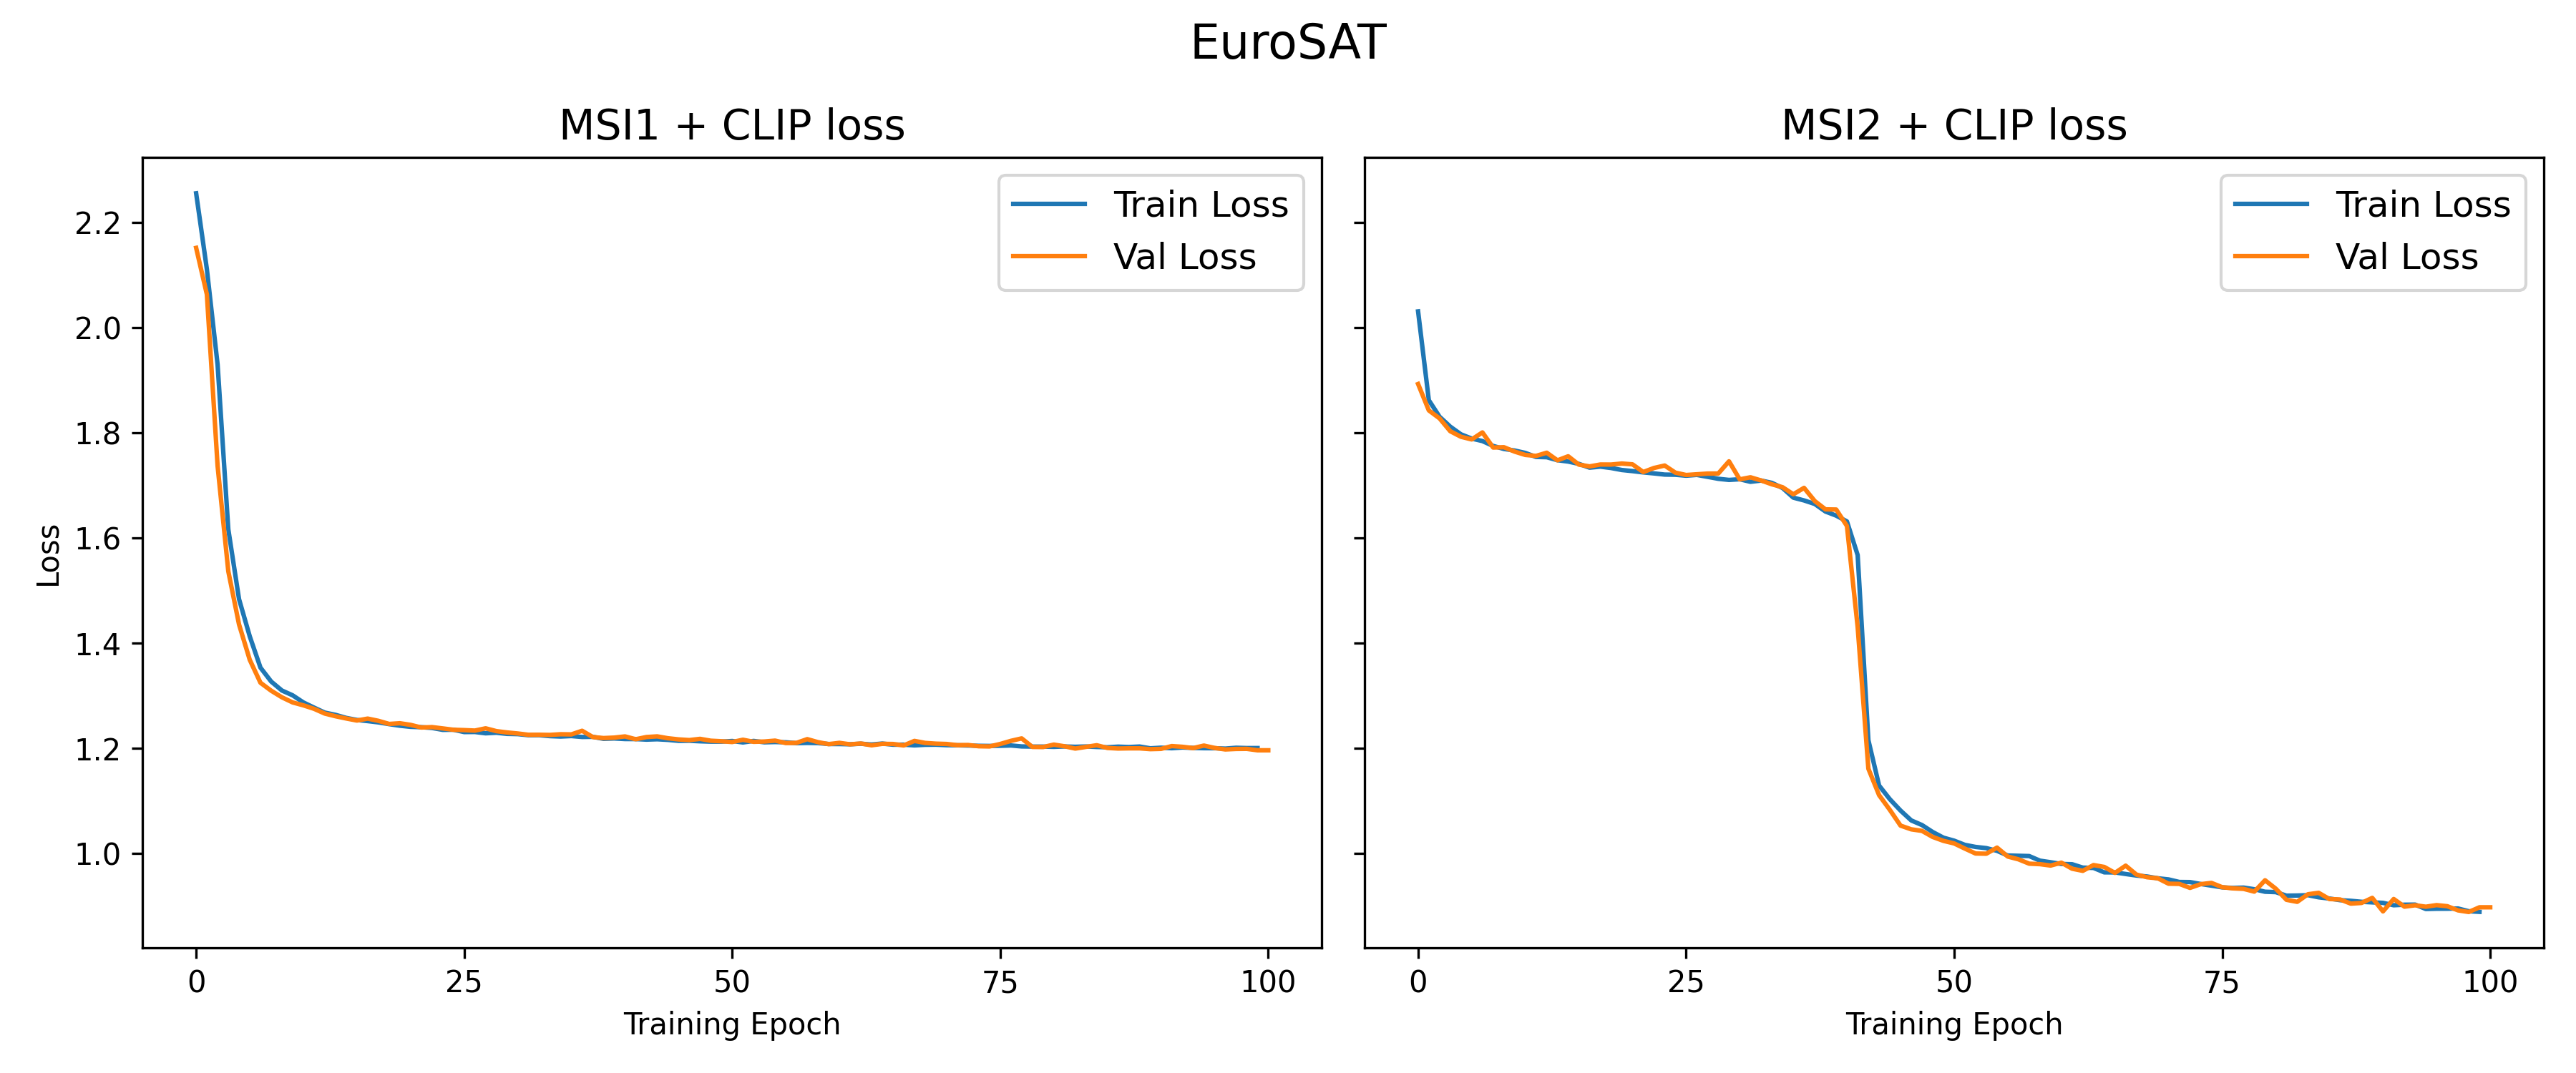
\includegraphics[width=\textwidth]{img/EuroSAT_loss_plot.png}
    \caption{Training and validation loss of the two embedders on the original EuroSAT dataset.}
    \label{fig:eurosatloss}
\end{figure}


\begin{figure}[h]
    \centering
    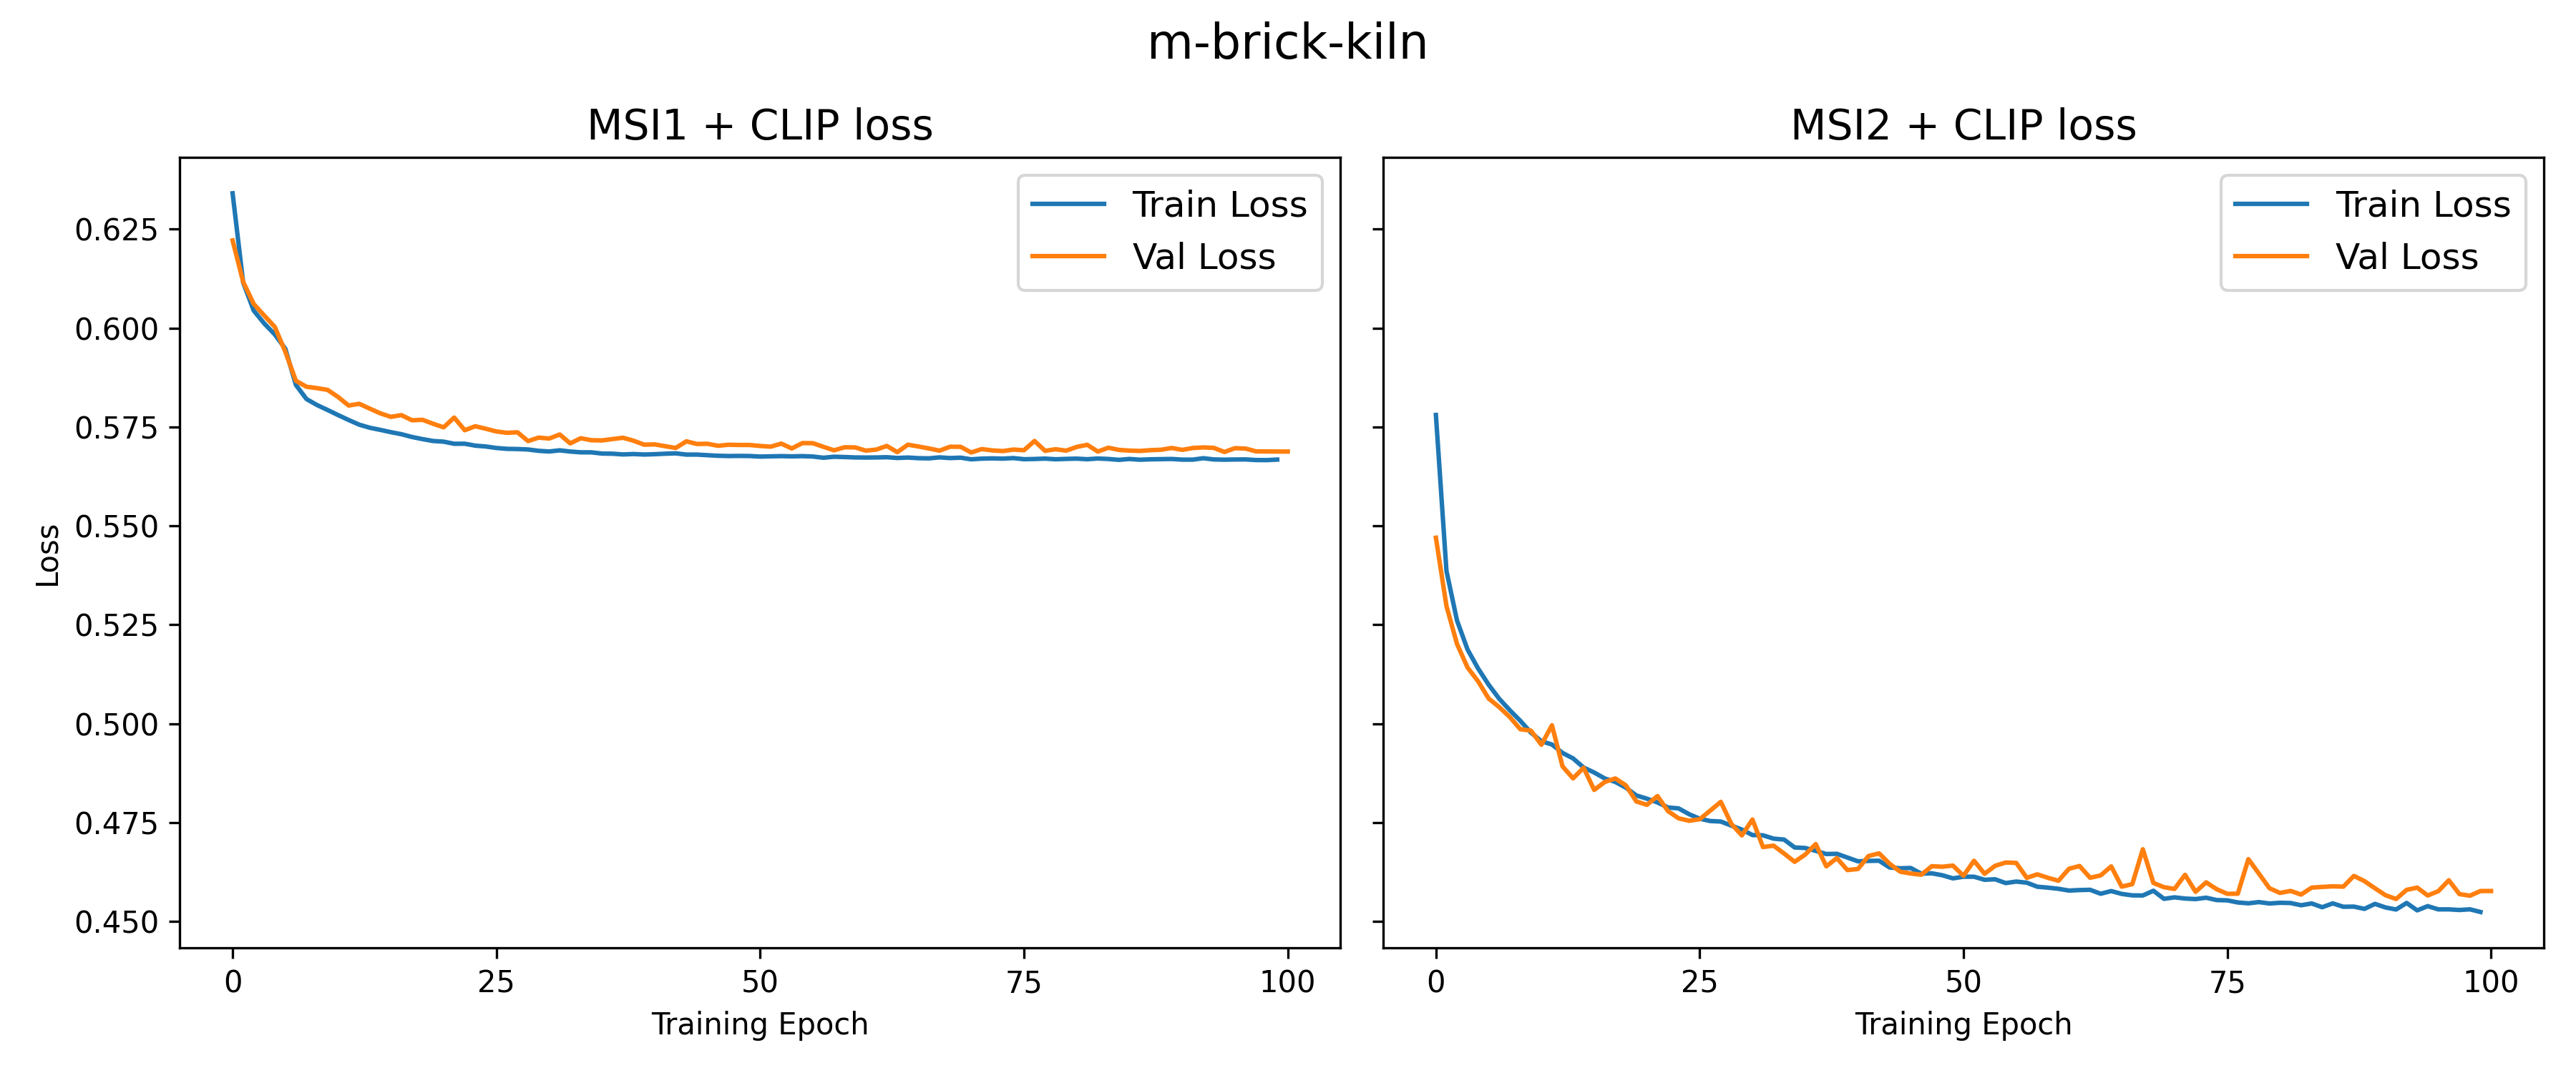
\includegraphics[width=\textwidth]{img/m-brick-kiln_loss_plot.png}
    \caption{Training and validation loss of the two embedders on the m-brick-kiln dataset from GEO-Bench.}
    \label{fig:brickloss}
\end{figure}

\begin{figure}[h]
    \centering
    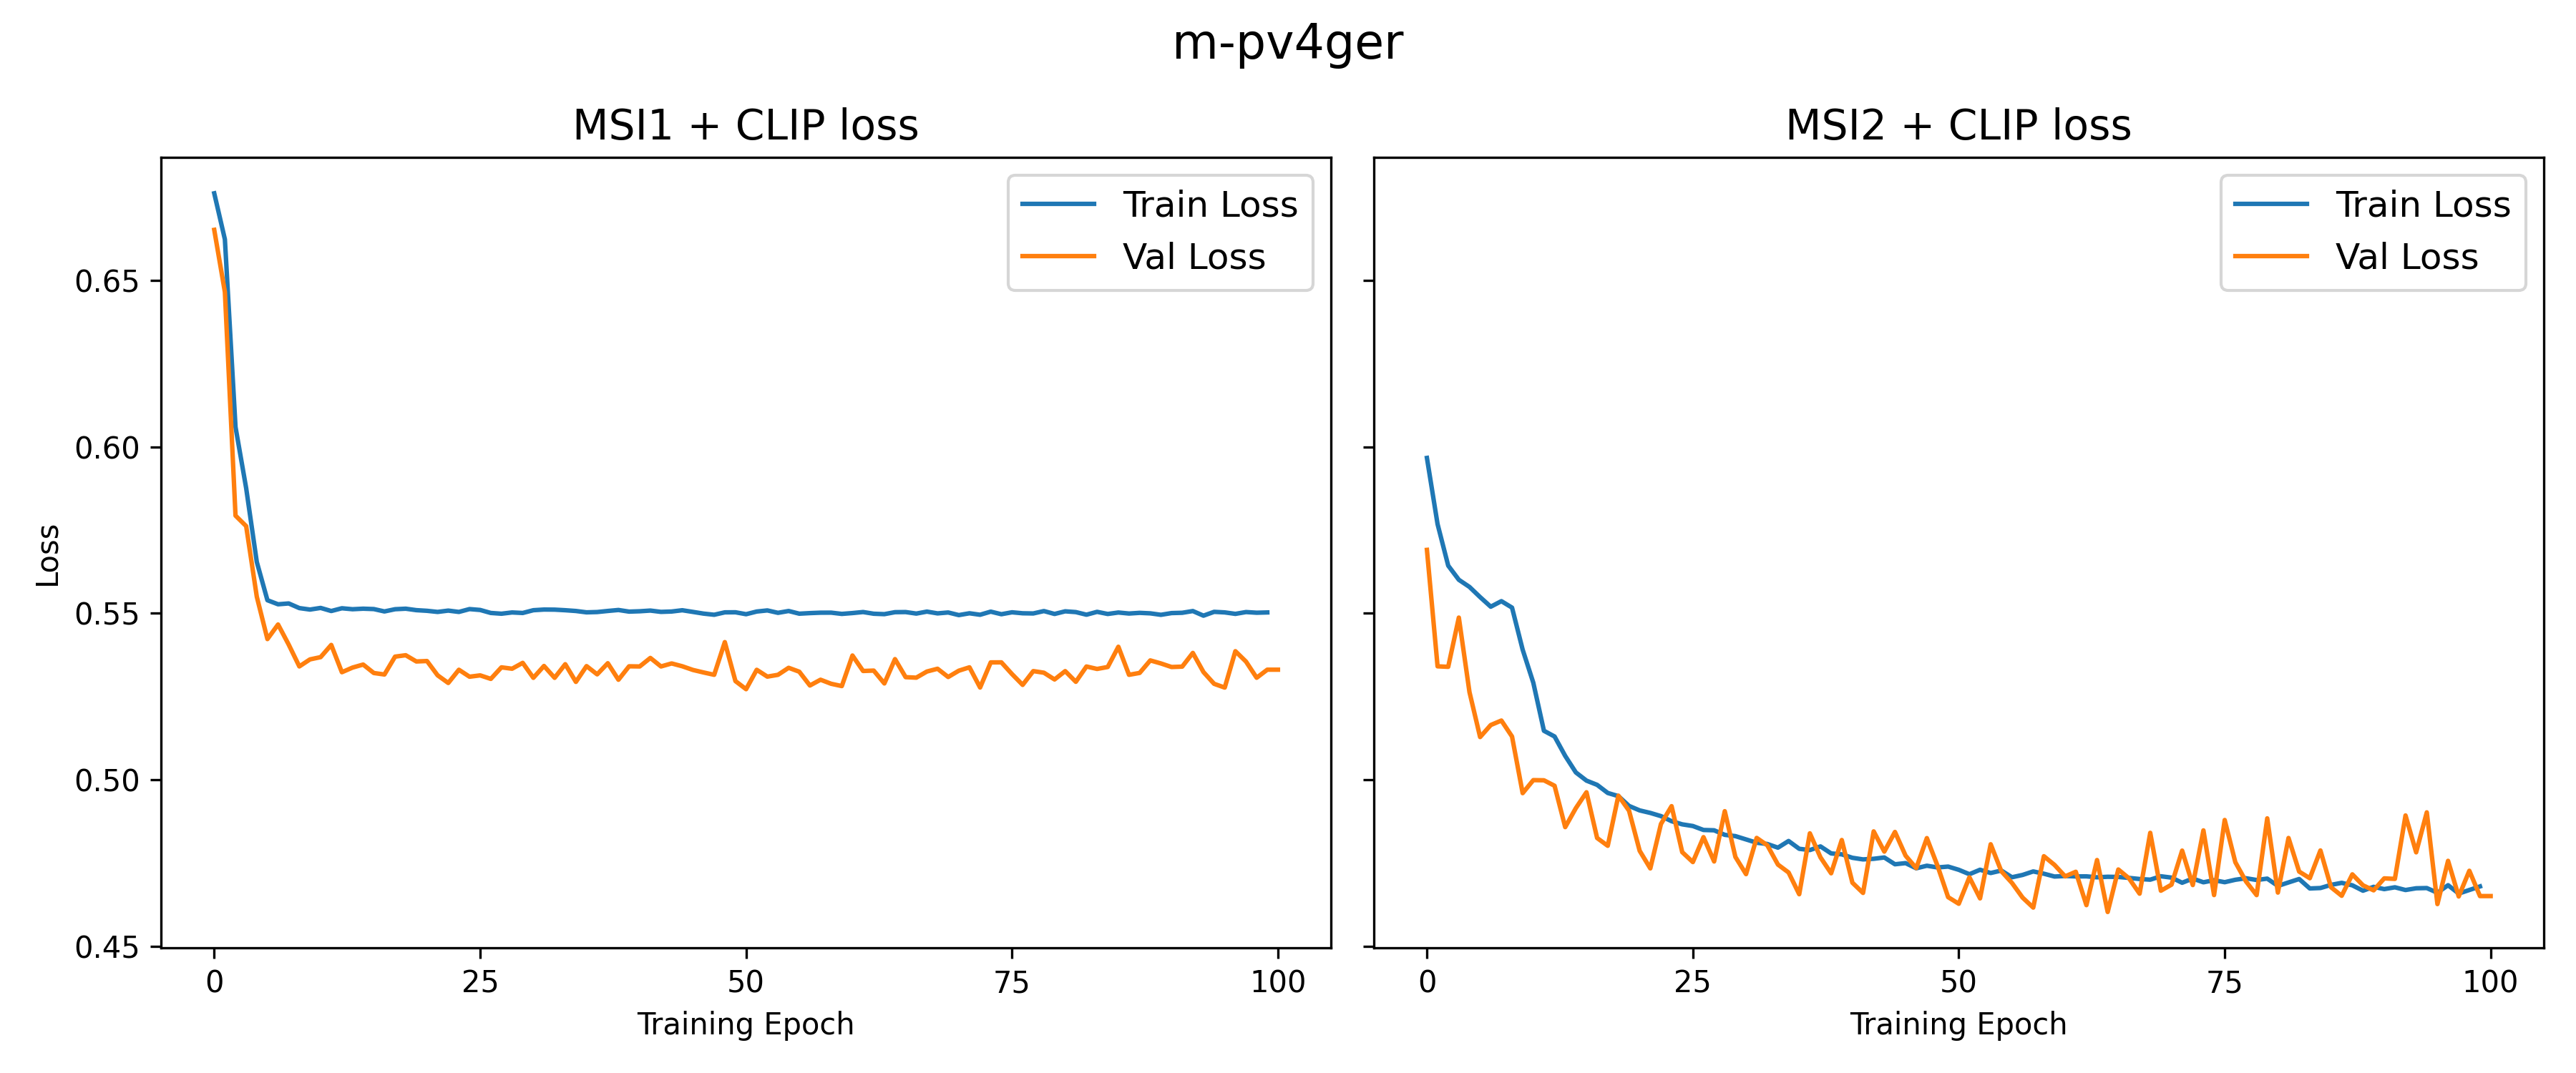
\includegraphics[width=\textwidth]{img/m-pv4ger_loss_plot.png}
    \caption{Training and validation loss of the two embedders on the m-pv4ger dataset from GEO-Bench.}
    \label{fig:solarloss}
\end{figure}

\begin{figure}[h]
    \centering
    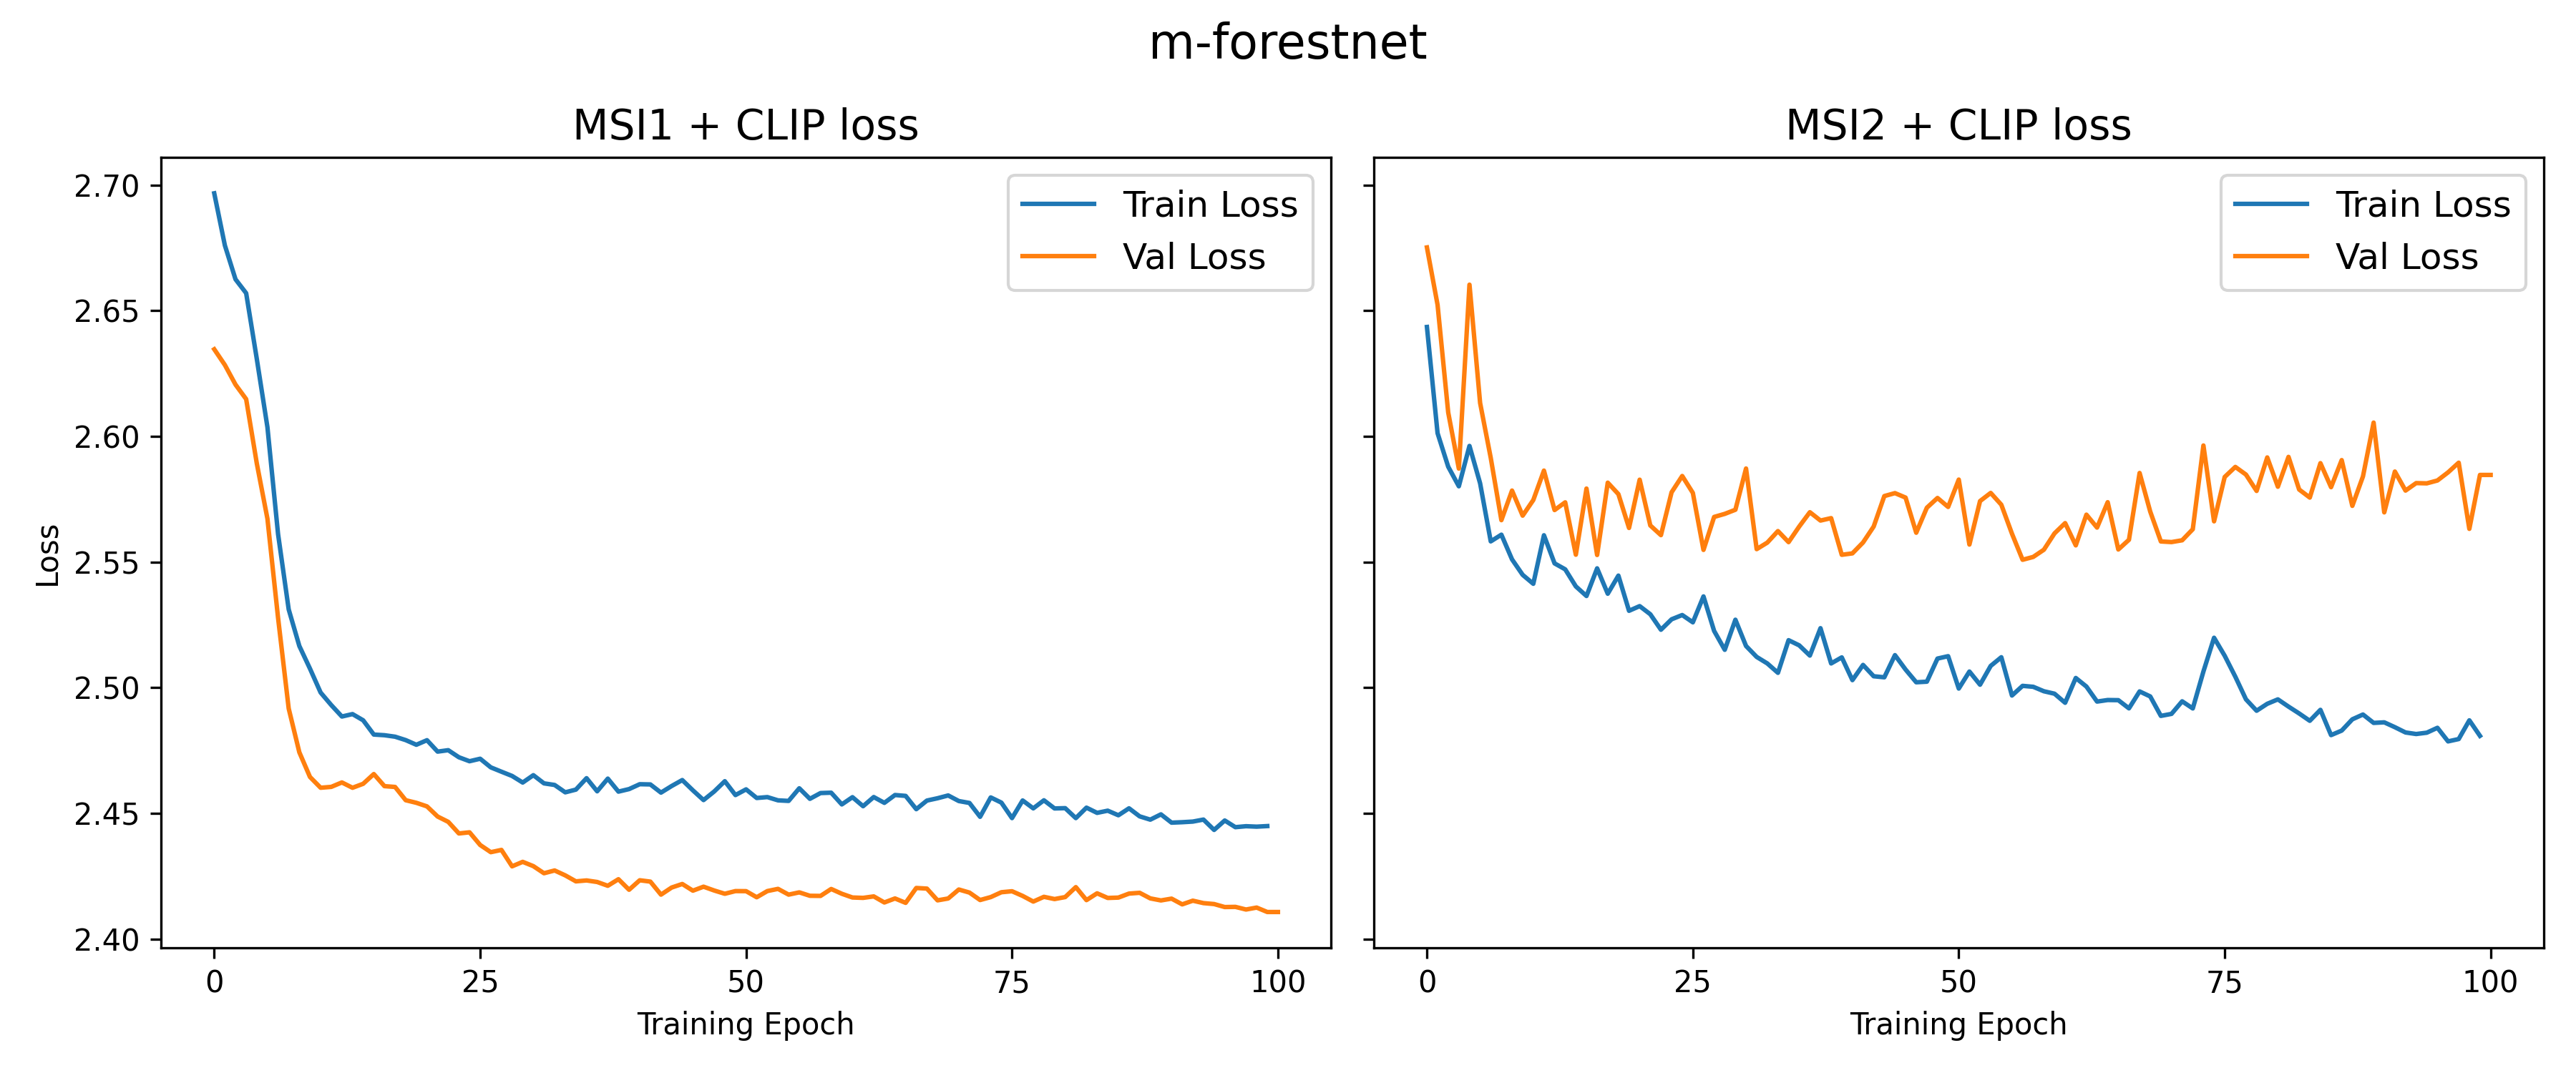
\includegraphics[width=\textwidth]{img/m-forestnet_loss_plot.png}
    \caption{Training and validation loss of the two embedders on the m-forestnet dataset from GEO-Bench.}
    \label{fig:foresloss}
\end{figure}

\begin{figure}[h]
    \centering
    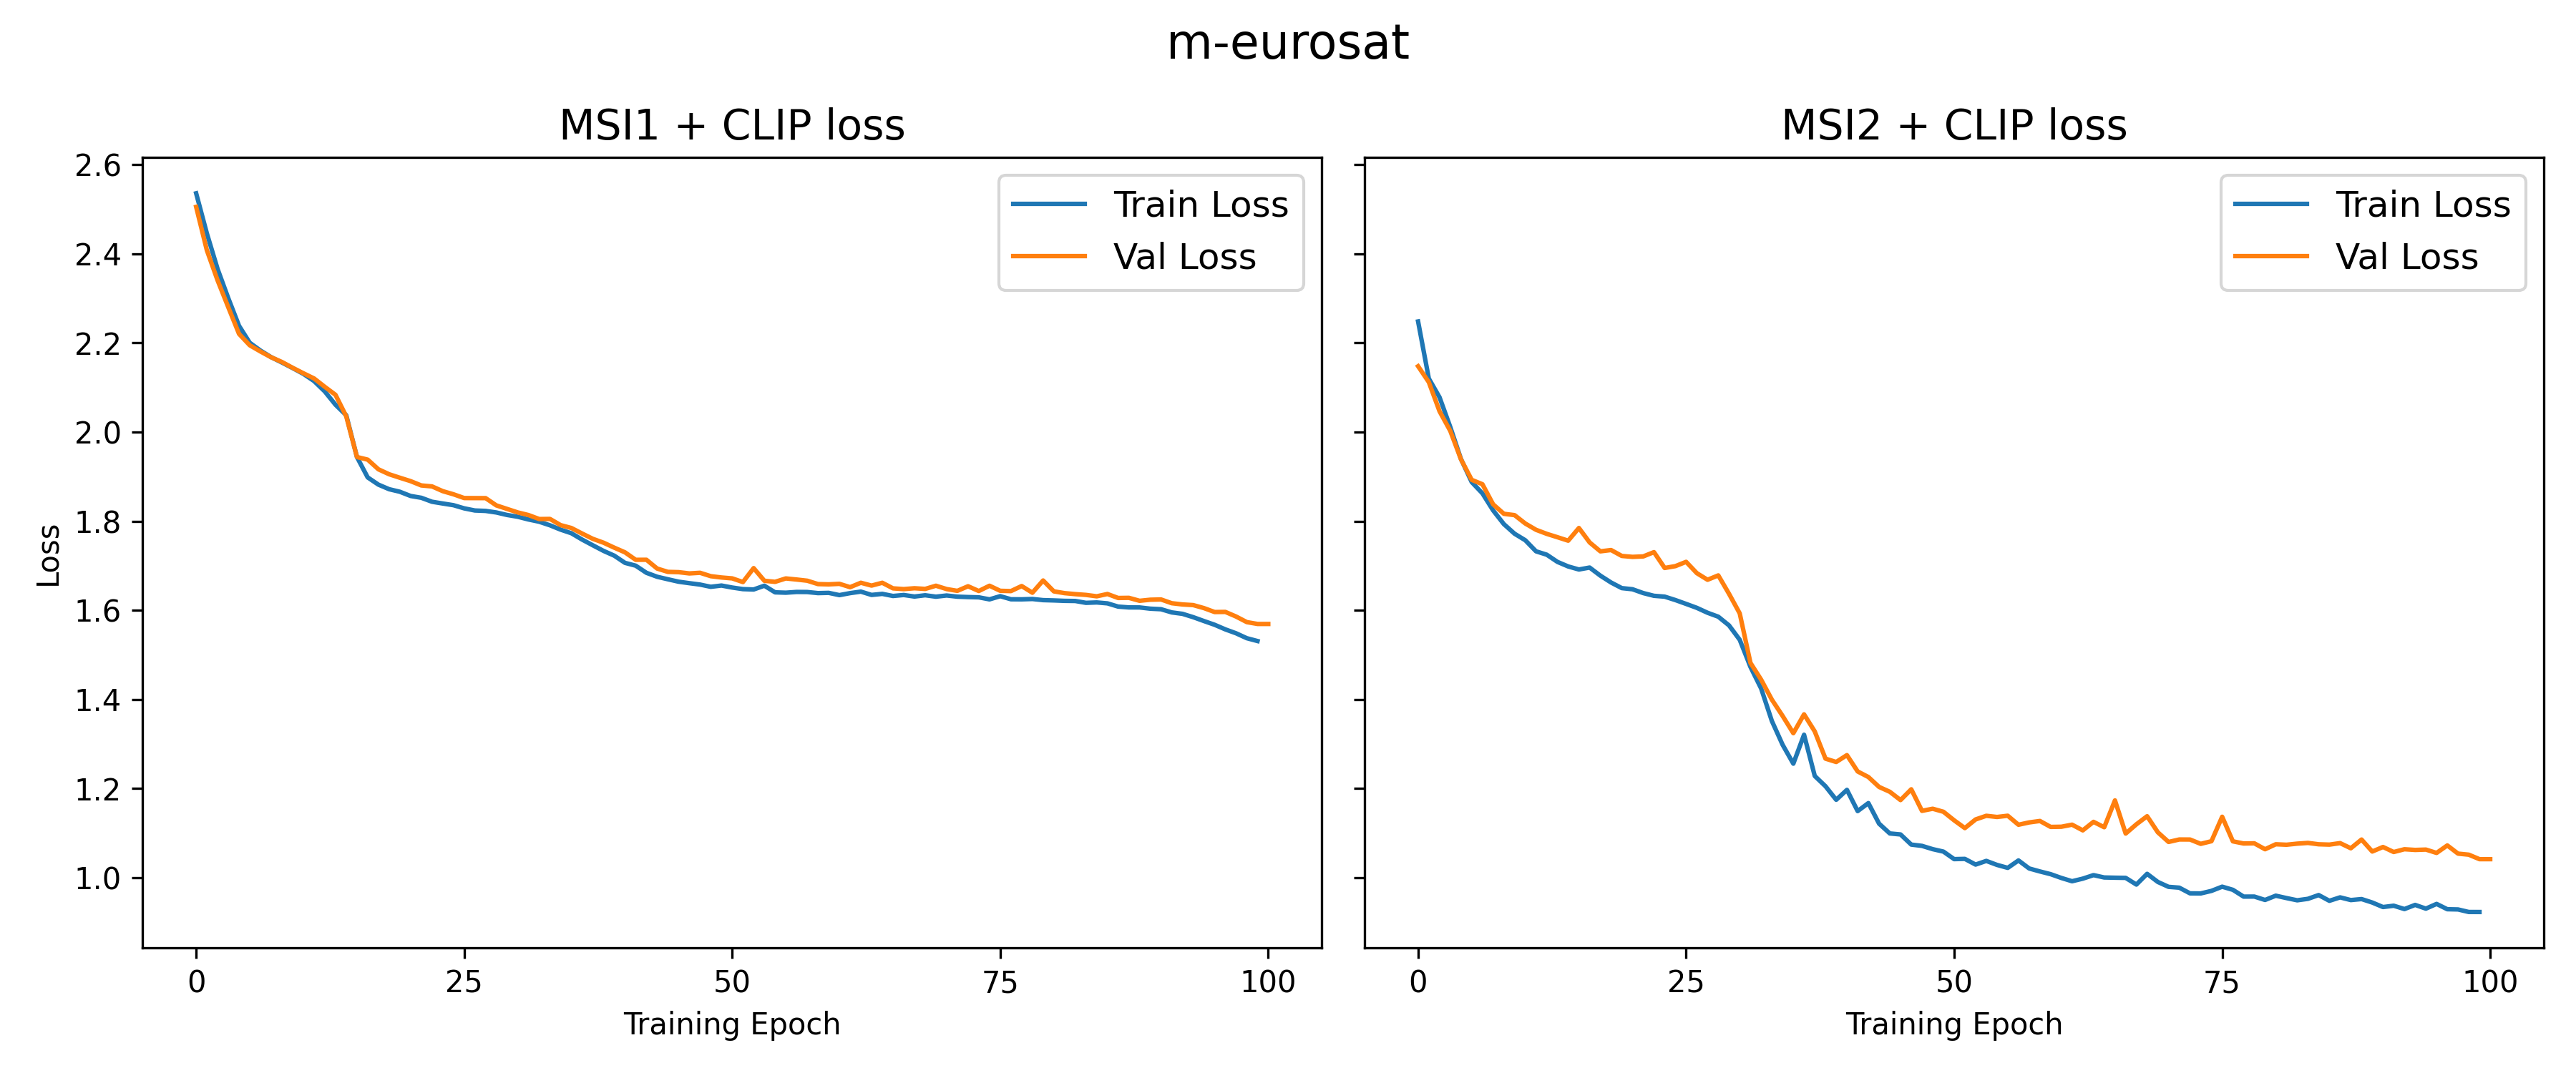
\includegraphics[width=\textwidth]{img/m-eurosat_loss_plot.png}
    \caption{Training and validation loss of the two embedders on the m-eurosat dataset from GEO-Bench.}
    \label{fig:meurosatloss}
\end{figure}

\begin{figure}[h]
    \centering
    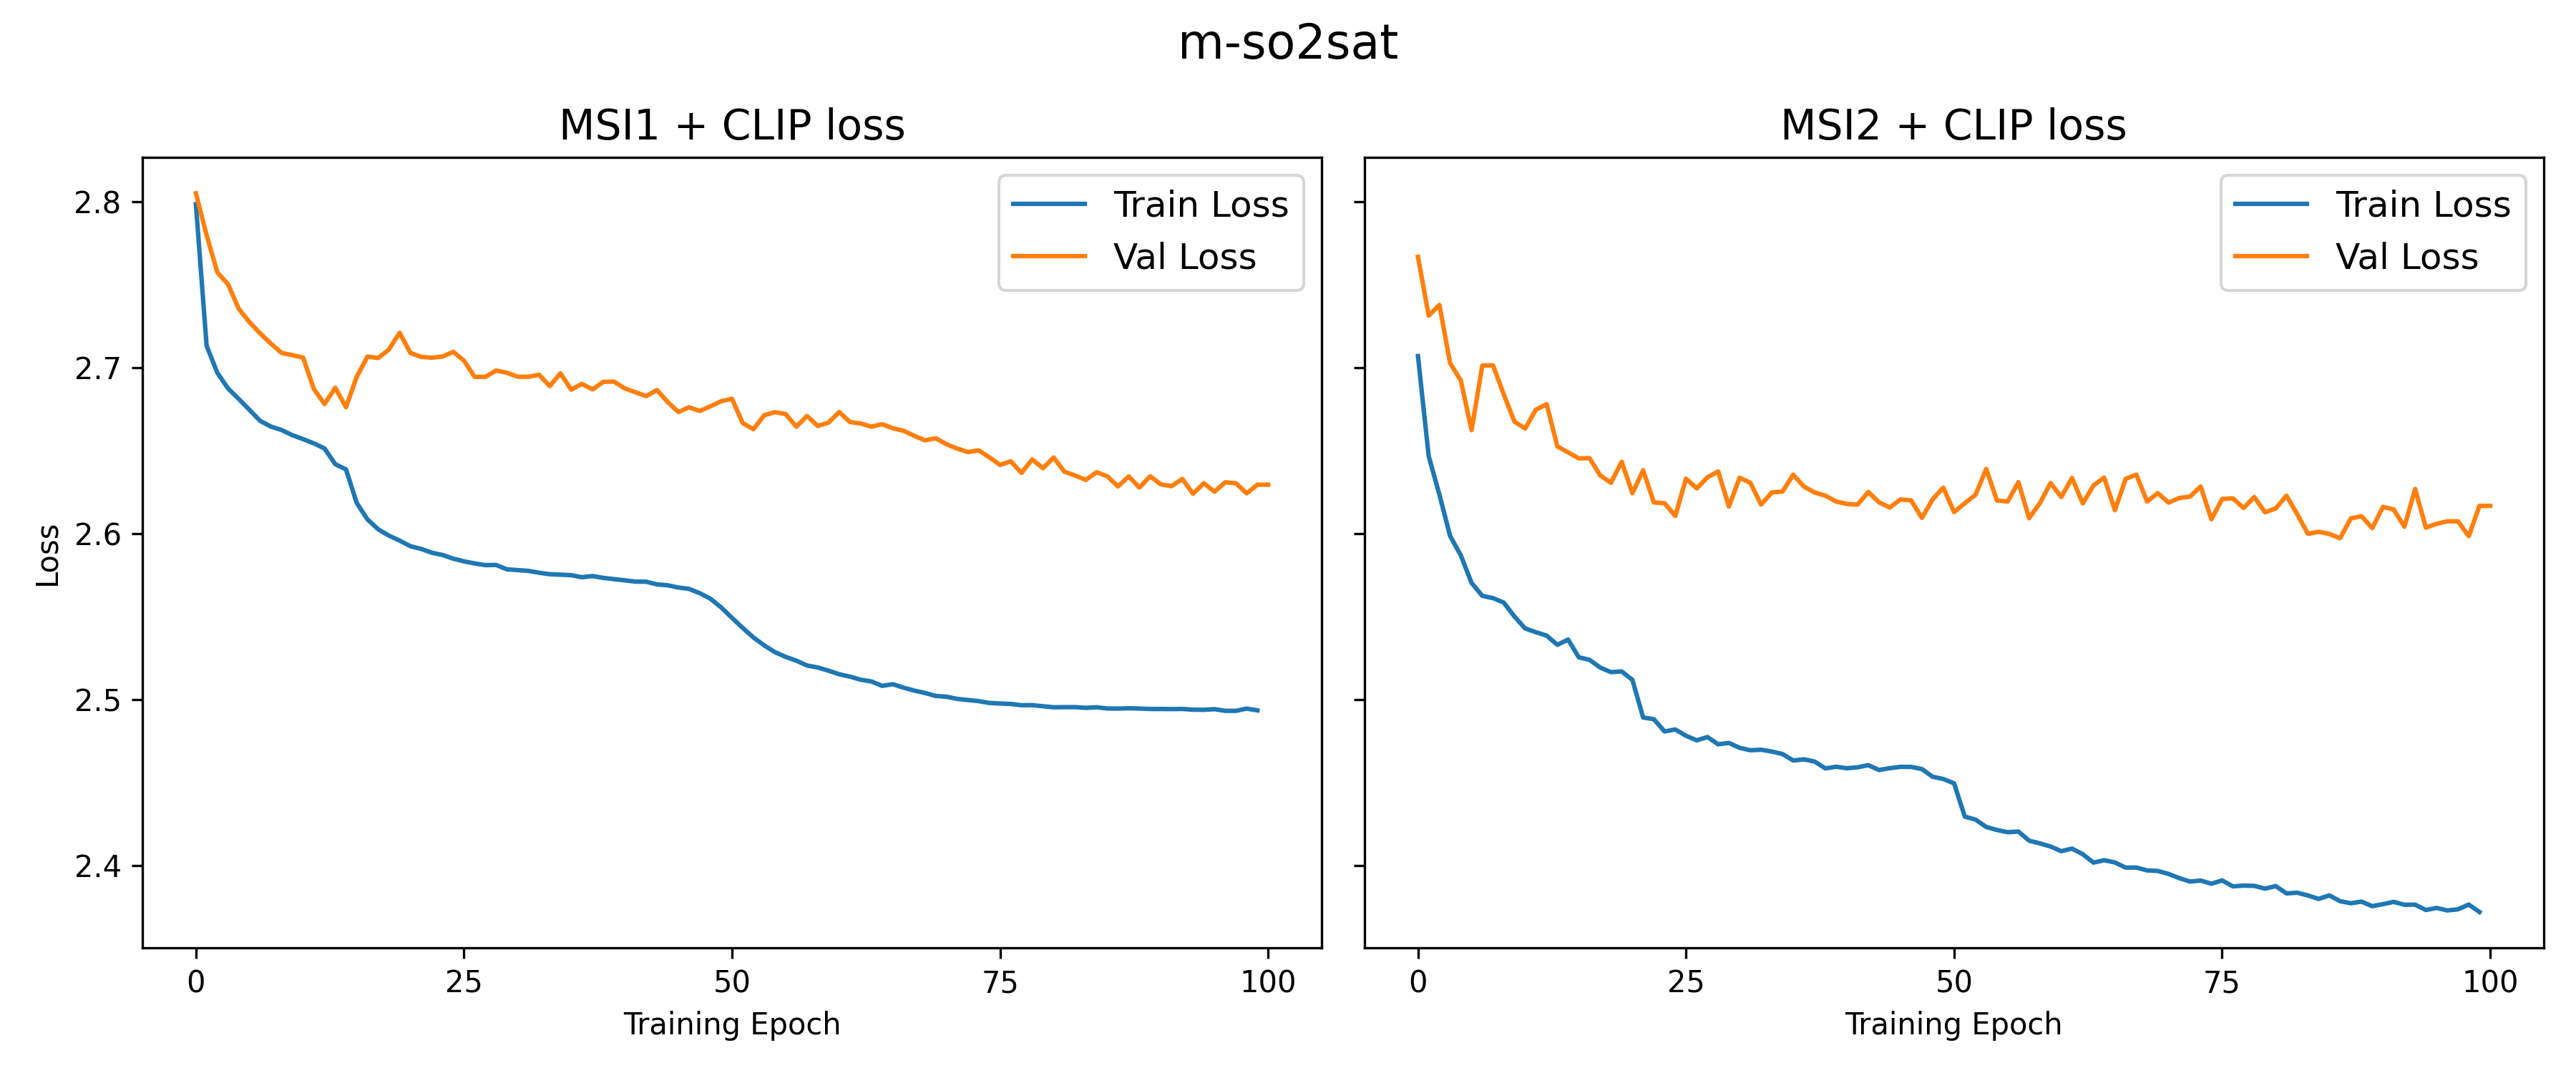
\includegraphics[width=\textwidth]{img/m-so2sat_loss_plot.png}
    \caption{Training and validation loss of the two embedders on the m-so2sat dataset from GEO-Bench.}
    \label{fig:so2satloss}
\end{figure}

\begin{figure}[h]
    \centering
    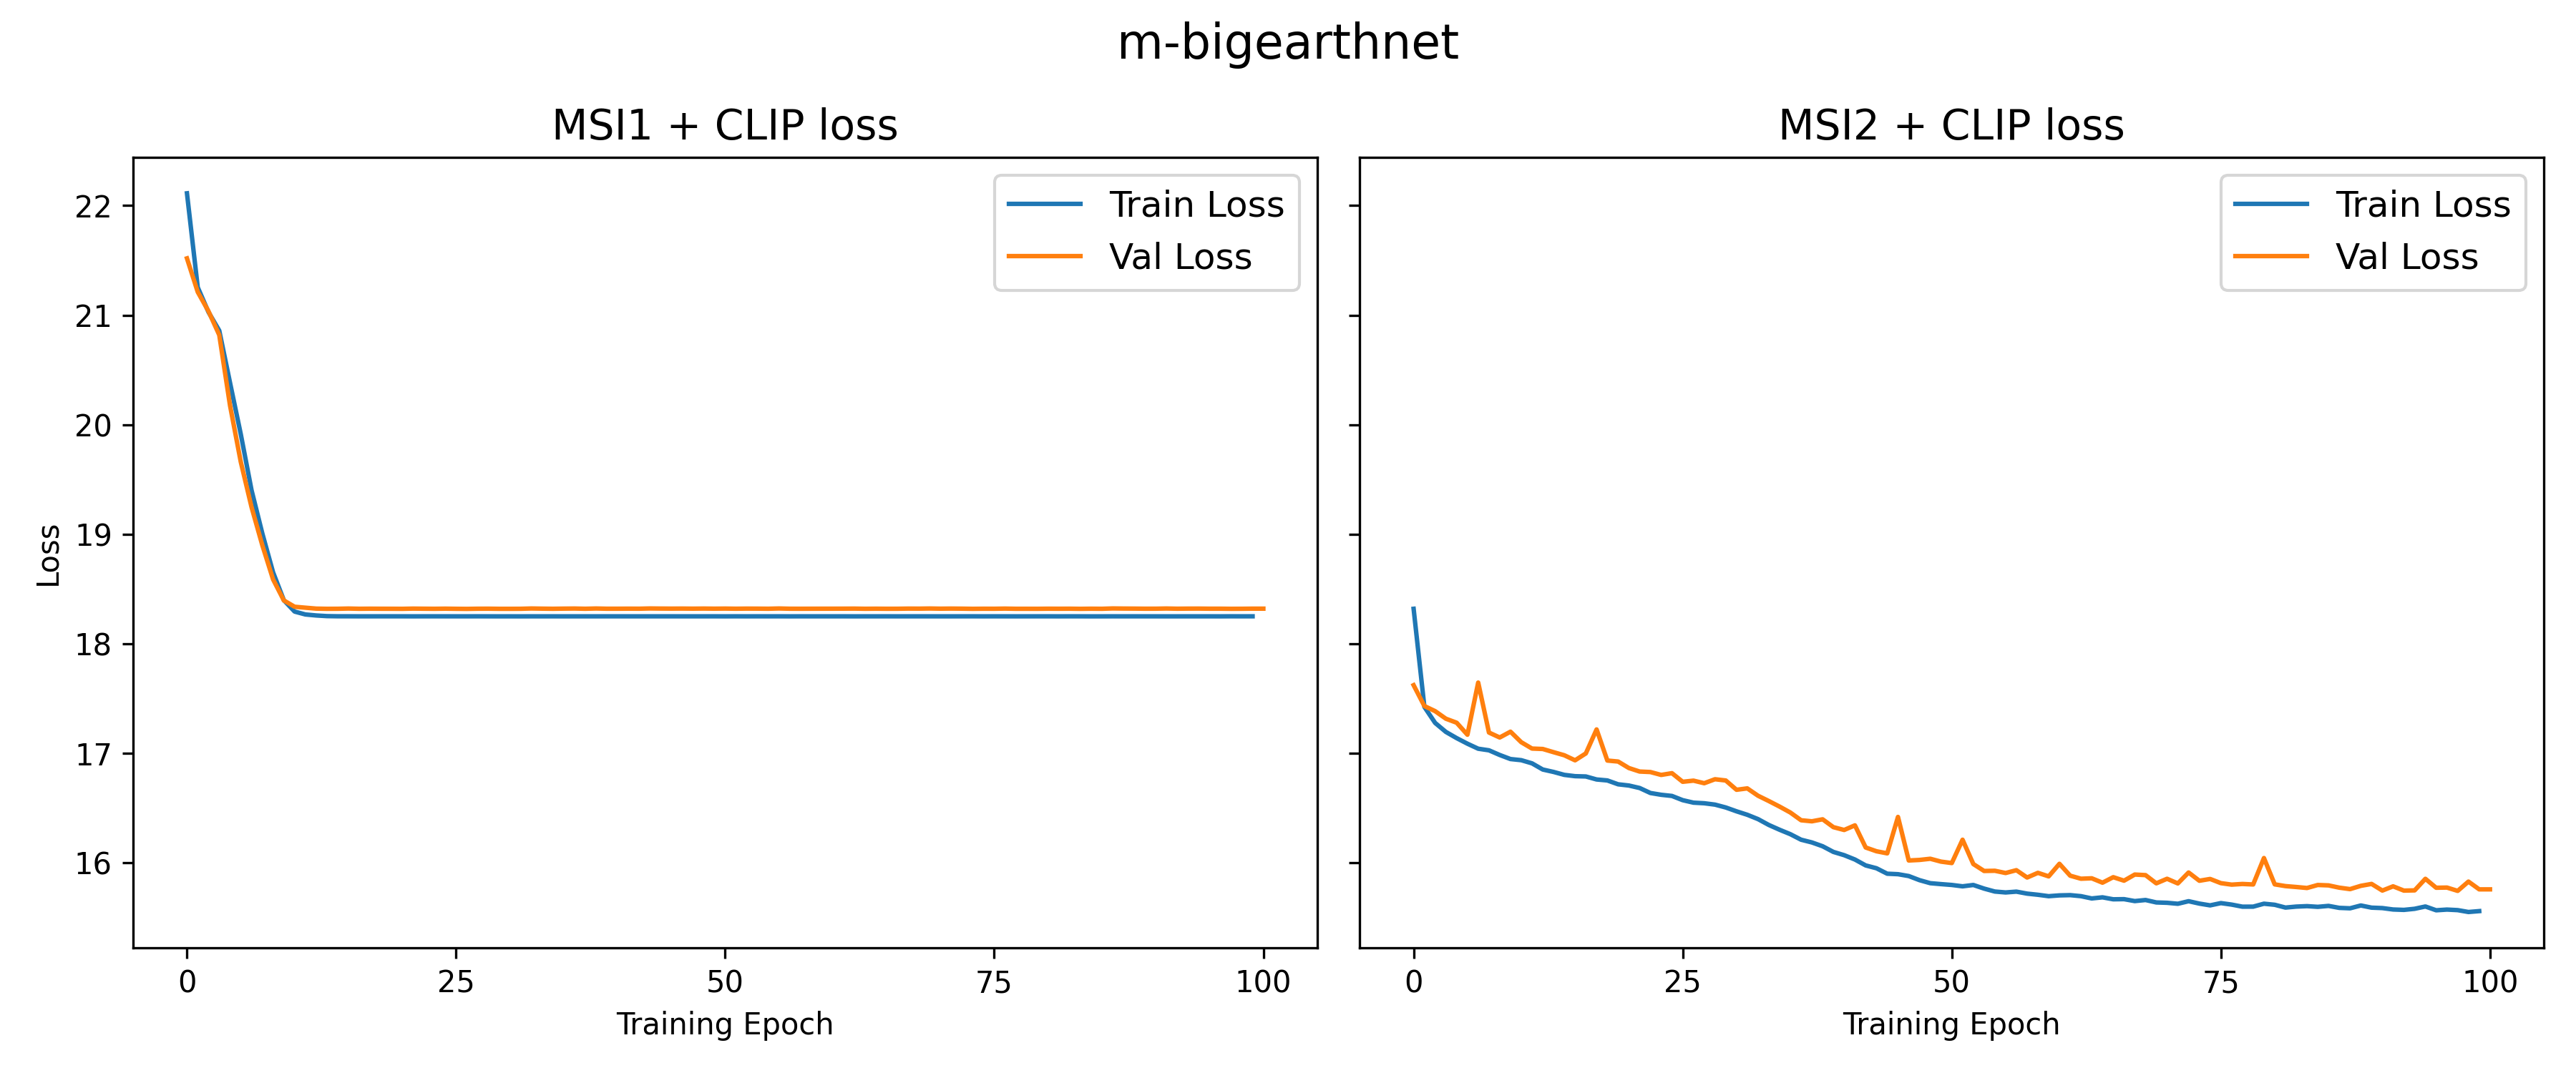
\includegraphics[width=\textwidth]{img/m-bigearthnet_loss_plot.png}
    \caption{Training and validation loss of the two embedders on the m-bigearthnet dataset from GEO-Bench.}
    \label{fig:benloss}
\end{figure}




\chapter{Conclusions} % ---------------------------------------
Conclusions on the work results, discussion of potential future directions (applying the MSI Embedder to a RS-specialized CLIP, trying different models, trying Open Vision)

Future work directions: hyperparameter tuning, trying bigger embedders, multilabel classification model to be restructured according to what said in that paper (maybe trying something like that with GeoRSCLIP or so, ...

Also see last chapters of the Pi School report


\backmatter
\cleardoublepage

% APPENDIX ----------------------------------------------------
\appendix
\chapter{Appendix}


\begin{table}[ht]
\centering
\footnotesize
\renewcommand{\arraystretch}{1.2}
    \begin{tabular}{cccccc|c}
    \toprule
    %\textbf{Model} & \textbf{Method} & \multicolumn{5}{c}{\textbf{m-bigearthnet}} \\
    \multirow{2}{*}{\textbf{Model}} & \multirow{2}{*}{\textbf{Method}} & \multicolumn{5}{c}{\textbf{m-bigearthnet}} \\
    \cmidrule(lr){3-7}
    & & \textbf{R@5} & \textbf{P@5} & \textbf{mAP} & \textbf{F1} & \textbf{rloss} \\
    \specialrule{.06em}{.2em}{.2em}
    CLIP & zero-shot & \textbf{31.70\%} &  \textbf{23.40\%} & \textbf{32.32\%} & \textbf{20.39\%} & \textbf{28.71\%} \\
    | &  | & | & | & | &| & | \\
    MSI1 & finetune & 19.99\% & 15.58\% & 24.57\% & 15.29\% & 39.82\% \\
    MSI2 & finetune & 15.58\% & 11.46\% & 19.44\% & 14.55\% & 45.53\% \\
    MSI-T-s & zero shot & 15.95\% & 12.84\% & 20.36\% & 16.46\% & 42.26\% \\
    MSI-T-E & zero shot & \underline{29.56\%1} & \underline{22.24\%} & \underline{30.90\%} & \underline{20.30\%} & \underline{28.58\%} \\
    MSI-T-E-4L & zero shot & 24.61\% & 19.02\% & 27.51\% & 19.23\% & 33.45\% \\
    \bottomrule
    \end{tabular}
\vspace{0.3cm}
\caption{\normalsize Performance of models on the m-bigearthnet dataset across various evaluation metrics.}
\label{tab:mbigearthnetresults}
\end{table}


% BIBLIOGRAPHY ------------------------------------------------
\newpage
\phantomsection % use this command only if hyperref is loaded
\addcontentsline{toc}{chapter}{\bibname}
% Here put the code for the bibliography. You can use BibTeX or
% the BibLaTeX package or the simple environment thebibliography.
\bibliographystyle{unsrt} % style can be changed
% 'unsrt' is identical to 'plain', but disables the automatic alphabetical order
\bibliography{references.bib}

\end{document}
